\documentclass[conference]{IEEEtran}

\usepackage{cite}
\usepackage{amsmath,amssymb,amsfonts}
\usepackage{graphicx}
\usepackage{booktabs}
\usepackage{multirow}
\usepackage{array}
\usepackage{url}
\usepackage{hyperref}
\usepackage{float}
\usepackage{xcolor}
\graphicspath{
  {images/clvit/}
  {images/mae/}
  {images/gradcam/}
}
\renewcommand\IEEEkeywordsname{Keywords}
\begin{document}

\title{
MAE-Pretrained Cross-Learning Vision Transformer\\
for Plant Disease Detection\\
\large A Two-Stage Self-Supervised and Supervised Deep Learning Pipeline
for Label-Efficient Plant Disease Classification
}

\author{
\IEEEauthorblockN{Jishan Aich, Devraj R B, Hansh Raj, Insaknok Pongen, Ranbir Singha}
\IEEEauthorblockA{
Department of Information Technology\\
North Eastern Hill University\\
Shillong, India\\
}
}

\maketitle

\begin{abstract}
This paper shows that a masked autoencoder (MAE), fused with a cross-attention fine-tuning architecture, is a label-efficient learner for plant disease classification. Our approach is two-staged: we first mask random patches of unlabelled leaf images and pretrain a Vision Transformer encoder to reconstruct the missing pixels, then we fine-tune the encoder under a Cross-Learning Vision Transformer (CLViT) that fuses two geometric views of each image via cross-attention and two auxiliary self-supervised prediction tasks. It is based on two core designs. First, we mask 75\% of input patches during pretraining, forcing the encoder to learn plant tissue structure and disease morphology from sparse observation rather than local interpolation. Second, we fuse an original and a geometrically transformed view of each image through cross-attention during fine-tuning, coupled with differential learning rates that protect the pretrained representation while the new modules adapt quickly. Coupling these two designs lets us train an effective classifier from a modest unlabelled corpus of 8,406 plant disease images: the frozen MAE encoder alone reaches 94.56\% linear probing accuracy with zero disease labels, and the fully fine-tuned CLViT reaches 99.83\% top-1 accuracy on a held-out test set of 1,802 images, with 100.00\% top-3 accuracy and only 3 total misclassifications. A label efficiency study shows our pipeline matches or exceeds a ViT-Base baseline pretrained on 14 million ImageNet-21k images, despite using three orders of magnitude fewer pretraining images. GradCAM analysis confirms the model attends predominantly to disease lesion regions rather than background, and we identify brightness sensitivity — attributable to the controlled-background acquisition protocol of the PlantVillage dataset — as the primary limitation for field deployment.
\end{abstract}
\vspace{0.5em}
\begin{IEEEkeywords}
Masked Autoencoder, Vision Transformer, Self-Supervised Learning,
Plant Disease Classification, Cross-Attention, Label Efficiency
\end{IEEEkeywords}

\section{Introduction}

Deep learning has driven rapid progress in automated plant disease diagnosis, with convolutional networks and, more recently, Vision Transformers (ViT)~\cite{3} reaching expert-level accuracy on benchmark datasets such as PlantVillage~\cite{2}. This progress has been coupled with a training strategy inherited from large-scale visual recognition: supervised pretraining on a labelled source domain, followed by fine-tuning on the target task. The resulting models are accurate under the conditions of their training data, but their adoption in real agricultural settings is constrained by one persistent bottleneck — the cost of expert-annotated labels. Identifying and labelling plant disease at the scale required for supervised training demands domain expertise that is scarce and expensive, particularly in the low-resource regions where automated diagnosis would be most valuable.
In this paper, we ask whether self-supervised pretraining on unlabelled plant images can reduce this dependence on labelled data without sacrificing accuracy. Our motivation follows directly from recent progress in self-supervised vision: masked image modelling ~\cite{1,9} and self-distillation ~\cite{7} have shown that a Vision Transformer pretrained without any label can learn representations that match or exceed supervised pretraining on transfer tasks. He et al.~\cite{1} show that masking a high proportion of an image—e.g., 75\%—and training an asymmetric encoder-decoder to reconstruct the missing pixels yields a non-trivial, meaningful self-supervisory task. Caron et al.~\cite{7} show that this kind of pretraining, when applied to ViT, produces features that are excellent k-NN classifiers without any fine-tuning. We adapt these findings to the plant disease domain, where the cost of supervision is the binding constraint rather than the scale of architecture.
We attempt to answer this question from two perspectives. First, we ask whether masked autoencoding—originally validated on ImageNet-scale natural images—transfers to a narrower, domain-specific corpus of plant disease images, where intra-class variability is lower but lesion-level detail is finer-grained than typical ImageNet categories. Second, we ask whether a pretrained encoder, once fine-tuned, can be made more label-efficient by introducing auxiliary self-supervised objectives directly into the supervised stage, rather than treating pretraining and fine-tuning as fully separate phases. This second question is motivated by the observation that rotation prediction~\cite{10} and other pretext tasks remain informative even when label-rich data is available, acting as a regulariser against overfitting on small labelled sets.
Driven by this analysis, we present a two-stage pipeline: a Masked Autoencoder (MAE) pretrained on unlabelled plant disease images, followed by a Cross-Learning Vision Transformer (CLViT) that fine-tunes the encoder under supervised classification while fusing two geometric views of each image through cross-attention. Unlike standard fine-tuning, which discards the pretrained encoder's self-supervised character once labels are introduced, CLViT keeps two auxiliary self-supervised prediction tasks active throughout fine-tuning, coupled with differential learning rates that protect the pretrained representation while new modules adapt. We show that this design produces a model that is competitive with a strong ImageNet-21k supervised baseline while requiring three orders of magnitude fewer pretraining images, and that the gap in its favour widens as the available label budget grows from 50\% to 100\% of the training set.


The primary contributions of this work are:

\begin{itemize}
\item \textbf{Domain-specific masked autoencoding.} We pretrain a ViT-B/16 encoder with a Masked Autoencoder on 8,406 unlabelled plant disease images at a 75\% masking ratio, and show via linear probing and t-SNE analysis that the resulting encoder learns biologically meaningful representations—including the correct unsupervised clustering of visually similar diseases caused by the same pathogen \textit{(Phytophthora infestans)}.
\item \textbf{Cross-Learning Vision Transformer (CLViT).} We introduce a fine-tuning architecture that fuses an original and a geometrically transformed view of each image through cross-attention, augmented by two auxiliary self-supervised heads (rotation and flip prediction) that remain active throughout supervised fine-tuning.
\item \textbf{Label efficiency analysis.} We evaluate CLViT and a supervised ViT-B/16 baseline pretrained on ImageNet-21k across four label fractions (10\%, 25\%, 50\%, 100\%) of the training set. CLViT matches or exceeds the baseline at 50\% and 100\% label availability, despite its pretraining corpus being three orders of magnitude smaller.
\item \textbf{Interpretability. }GradCAM analysis shows that CLViT attends predominantly to disease-relevant leaf regions, and we identify a specific background co-activation pattern that explains the model's reduced robustness to brightness perturbation.

The remainder of this paper is organised as follows. Section 2 reviews related work in self-supervised vision and plant disease detection. Section 3 describes the methodology. Section 4 details the experimental setup. Section 5 presents results. Section 6 discusses findings, Section 7 states limitations and future work, and Section 8 concludes.
\end{itemize}

\section{Related Work}

\subsection{Plant Disease Detection with Deep Learning}

Mohanty et al.~\cite{14} established the PlantVillage benchmark and demonstrated that deep CNNs can classify 26 diseases across 14 crop species with over 99\% accuracy under controlled conditions. Subsequent work identified the domain shift problem: models trained on PlantVillage perform poorly on field-collected images~\cite{18}, motivating research into domain adaptation and data augmentation for agricultural imaging.
Attention-based CNN architectures~\cite{16} have been applied to localise disease regions within leaves, improving both accuracy and interpretability. Transformer architectures were introduced to plant pathology by Saleem et al.~\cite{21}, who demonstrated that ViT fine-tuned from ImageNet pretraining outperforms CNN counterparts on several agricultural benchmarks. However, these approaches rely entirely on supervised pretraining and do not exploit the large pool of unlabelled plant images available in practice


\subsection{Self-Supervised Learning for Vision}

Contrastive self-supervised methods [SimCLR, MoCo v2, v3~\cite{8}] learn representations by maximising agreement between augmented views of the same image. These methods achieve strong transfer performance but require large batch sizes and careful augmentation design. Self-distillation methods such as DINO~\cite{7} use momentum encoders and patch-level token alignment, achieving particularly strong local feature learning. These methods do not produce pixel-level reconstruction and are not directly applicable to the patch reconstruction objective used in the present work.
Masked image modelling was introduced in the vision domain by BEiT ~\cite{20}, which predicts discrete visual tokens for masked patches. SimMIM~\cite{9} simplifies this by predicting raw pixel values without tokenisation. MAE~\cite{1} demonstrates that a lightweight decoder is sufficient for pretraining a high-quality encoder, and that per-patch normalised MSE loss outperforms raw pixel prediction. The present work adopts MAE as the Stage 1 pretraining framework for its simplicity, computational efficiency, and demonstrated superiority under limited data regimes.


\subsection{Vision Transformers in Agriculture}

The application of ViTs to agricultural imaging remains relatively underexplored compared to CNNs. Existing work has applied pre-trained ViTs (DeiT, Swin Transformer) to crop disease classification via standard supervised fine-tuning~\cite{21}. To our knowledge, the present work is the first to apply domain-specific MAE pretraining to plant disease images and to combine the pretrained encoder with an auxiliary SSL fine-tuning architecture specifically designed for the agricultural imaging domain.

\subsection{Auxiliary Self-Supervised Tasks}

The use of geometric prediction tasks as auxiliary SSL objectives during supervised fine-tuning was established by RotNet~\cite{10}, which demonstrated that rotation prediction is an effective pretext task for learning orientation-invariant features. Multi-task learning with SSL auxiliary objectives has been applied in medical imaging~\cite{22} to improve generalisation under label scarcity. The cross-attention fusion between two geometric views in CLViT is conceptually related to cross-view prediction in contrastive learning [SimCLR, BYOL], but is applied as an architectural component within supervised fine-tuning rather than as a standalone pretraining objective.

\section{Methodology}

\subsection{Overview}
The pipeline consists of two sequential training stages.
\begin{enumerate}
\item MAE Pretraining
\item CLViT Fine-Tuning
\end{enumerate}
Stage 1 trains a Masked Autoencoder on the full image corpus without class labels. The encoder learns representations of plant tissue structure, vein morphology, and disease lesion patterns through a self-supervised patch reconstruction pretext task. Stage 2 transfers the pretrained encoder to CLViT, which fine-tunes it under supervised classification augmented with geometric auxiliary SSL tasks and cross-attention fusion between dual views of each training image.



\subsection{Dataset}

Experiments use a six-class subset of PlantVillage [2] comprising 12,009 images: potato early blight, potato healthy, potato late blight, tomato early blight, tomato healthy, and tomato late blight. The dataset is partitioned once (seed = 42) into training (70\%, n = 8,406), validation (15\%, n = 1,801), and test (15\%, n = 1,802) subsets. Partition indices are serialised and reused identically across all scripts. The test set is accessed exactly once after all training decisions are finalised.

\begin{table}[H]
\centering
\caption{\textit{Per-class image counts}}
\begin{tabular}{lcccc}
\toprule
Class & Total & Train & Val & Test\\
\midrule
Potato Early & 1998 & 1418 & 291 & 289\\
Potato Healthy & 2008 & 1399 & 311 & 298\\
Potato Late & 1998 & 1396 & 284 & 318\\
Tomato Early & 1998 & 1408 & 289 & 301\\
Tomato Healthy & 2003 & 1388 & 317 & 298\\
Tomato Late & 2004 & 1397 & 309 & 298\\
\midrule
Total & 12009 & 8406 & 1801 & 1802\\
\bottomrule
\end{tabular}
\end{table}

\subsection{MAE Pretraining}
\subsubsection{\textit{\textbf{Architecture}}}
The MAE adopts an asymmetric encoder-decoder. The encoder is ViT-B/16~\cite{3}: patch size 16×16, 224×224 input (196 tokens), embedding dimension d = 768, 12 transformer blocks, 12 heads, ~86 M parameters, fixed 2D sine-cosine positional embeddings. The decoder is lightweight: 4 blocks, dimension 512, 8 heads, learned positional embeddings. The decoder is discarded after pretraining.
The encoder uses ViT-B/16 architecture.
\vspace{0.5em}
\subsubsection{\textit{\textbf{Masking and Reconstruction Objective}}}
Masking ratio $\rho = 0.75$ removes 147 of 196 patches per image per step, leaving 49 visible. Mask tokens are not introduced at the encoder stage, eliminating the pretraining/deployment distribution gap. The reconstruction target uses per-patch layer normalisation:
\begin{equation}
\hat{x}
=
\frac{x_i-\mu_{patch}}
{\sqrt{\sigma^2_{patch}+10^{-6}}}
\end{equation}


The reconstruction objective is

\begin{equation}
L_{\mathrm{MAE}}
=
\frac{1}{|M|}
\sum_{i \in M}
\left\|
\frac{x_i-\mu_{patch}}
{\sqrt{\sigma^2_{patch}+10^{-6}}}
-
\hat{x}_i
\right\|_2^2
\end{equation}

Where:

\begin{equation}
\mu_i=\frac{1}{P}\sum_{j=1}^{P}x_{ij}
\end{equation}

\begin{equation}
\sigma_i^2=\frac{1}{P}\sum_{j=1}^{P}(x_{ij}-\mu_i)^2
\end{equation}

where $M$ denotes the set of masked patches, $x_i$ and
$\hat{x}_i$ represent the normalized target patch and its
reconstruction, respectively, $\mu_i$ and $\sigma_i^2$
denote the mean and variance of patch $i$, $P$ is the
number of pixel values in each patch, and $\epsilon$
is a small constant used for numerical stability.

\subsubsection{\textit{\textbf{Training}}}

Pretraining runs for 800 epochs (batch size 64, effective learning rate
$3.75 \times 10^{-5}$ via the linear scaling rule~\cite{5},
cosine decay with a 40-epoch warmup, AdamW
($\beta_1 = 0.9$, $\beta_2 = 0.95$),
weight decay 0.05, automatic mixed precision (AMP),
and gradient clipping of 1.0.

Data augmentation is minimal, consisting of
\texttt{RandomResizedCrop} with an output size of
$224 \times 224$ and a scale range of $0.2$--$1.0$,
followed by random horizontal flipping and
ImageNet normalization.

\subsection{Cross-Learning Vision Transformer}

\subsubsection{\textit{\textbf{Dual-View Encoding}}}
For each training batch, two views are constructed. The original
view $x$ uses the standard fine-tuning augmentation pipeline.
A transformed view $x'$ additionally applies a random rotation
$\theta \in \{0^\circ, 90^\circ, 180^\circ, 270^\circ\}$ and a
horizontal flip $\phi \in \{0,1\}$, applied on CPU-resident tensors
for numerical stability. Both views are processed by the same shared
encoder without masking. The resulting global representations are
obtained by mean-pooling:

\begin{equation}
z_{\mathrm{orig}}=
\frac{1}{196}
\sum_{i=1}^{196}
h_{\mathrm{orig}}[i],
\qquad
z_{\mathrm{trans}}=
\frac{1}{196}
\sum_{i=1}^{196}
h_{\mathrm{trans}}[i].
\end{equation}

\subsubsection{\textit{\textbf{Cross-Attention Fusion}}}

The original view (query) attends to the transformed view (key/value):

\begin{equation}
\begin{aligned}
A
&=
\mathrm{Dropout}\Big(
\mathrm{Proj}\big(
\mathrm{MHA}( \\
&\qquad
\mathrm{LN}(z_{\mathrm{orig}}),
\mathrm{LN}(z_{\mathrm{trans}}),
\mathrm{LN}(z_{\mathrm{trans}})
)
\big)
\Big)
\end{aligned}
\end{equation}

where $z_{\mathrm{orig}}, z_{\mathrm{trans}} \in \mathbb{R}^{768}$ are the global representations of the original and transformed views, respectively. $\mathrm{LN}(\cdot)$ denotes Layer Normalization, $\mathrm{MHA}(\cdot)$ denotes the multi-head cross-attention operation, $\mathrm{Proj}(\cdot)$ is a learnable linear projection, and $\mathrm{Dropout}(\cdot)$ is applied with a dropout rate of $0.1$.

\begin{equation}
c=\mathrm{FusionNorm}\!\left(
\mathrm{FusionProj}
\left(
\mathrm{cat}\left[z_{\mathrm{orig}},A\right]
\right)
\right),
\qquad
c\in\mathbb{R}^{768}
\end{equation}

where $\mathrm{cat}[\cdot,\cdot]$ denotes channel-wise feature concatenation, $\mathrm{FusionProj}:\mathbb{R}^{1536}\rightarrow\mathbb{R}^{768}$ represents a learnable projection implemented as a Linear $\rightarrow$ GELU $\rightarrow$ Dropout($0.1$) block, and $\mathrm{FusionNorm}$ denotes Layer Normalization applied after the projection.


\subsubsection{\textit{\textbf{Task Heads and Loss}}}

Three heads operate on $c$:

\begin{equation}
h_{\mathrm{cls}}:\mathbb{R}^{768}\rightarrow\mathbb{R}^{6}
\end{equation}

\begin{equation}
h_{\mathrm{rot}}:\mathbb{R}^{768}\rightarrow\mathbb{R}^{4}
\end{equation}

\begin{equation}
h_{\mathrm{flip}}:\mathbb{R}^{768}\rightarrow\mathbb{R}^{2}
\end{equation}

\begin{equation}
L
=
L_{\mathrm{CE}}(h_{\mathrm{cls}},y)
+
0.3\,L_{\mathrm{CE}}(h_{\mathrm{rot}},r)
+
0.2\,L_{\mathrm{CE}}(h_{\mathrm{flip}},f)
\end{equation}

where $h_{\mathrm{cls}}$ denotes the disease classification head, $h_{\mathrm{rot}}$ denotes the rotation prediction head, and $h_{\mathrm{flip}}$ denotes the horizontal flip prediction head. $L_{\mathrm{CE}}$ represents the cross-entropy loss, while $y$, $r$, and $f$ denote the ground-truth labels for disease classification, rotation prediction, and flip prediction, respectively. The weighting factors are $\lambda_{\mathrm{rot}}=0.3$ and $\lambda_{\mathrm{flip}}=0.2$. All heads use label smoothing with $\epsilon=0.1$.

\vspace{0.5em}

\subsubsection{\textit{\textbf{Differential Learning Rates}}}

Differential learning rates prevent catastrophic forgetting~\cite{12}. The encoder is optimized with a learning rate of $\mathrm{lr}_{\mathrm{encoder}}=3\times10^{-5}$, while the newly introduced classification heads and fusion module are optimized with $\mathrm{lr}_{\mathrm{heads+fusion}}=3\times10^{-4}$, as shown in (\ref{eq:lr}).

The model is optimized using AdamW with $\beta_{1}=0.9$ and $\beta_{2}=0.999$, employing a cosine learning-rate decay schedule with a 5-epoch warmup. Training is performed for 100 epochs using a batch size of 32 and a weight decay of 0.05. Automatic Mixed Precision (AMP) is utilized to accelerate training, and gradient clipping with a maximum norm of 1.0 is applied to improve optimization stability. The final model is selected based on the highest validation accuracy.

\begin{equation}
\mathrm{lr}_{\mathrm{encoder}} = 3 \times 10^{-5},
\qquad
\mathrm{lr}_{\mathrm{heads+fusion}} = 3 \times 10^{-4}
\label{eq:lr}
\end{equation}

\section{Experimental Setup}

\subsection{Hardware and Software}

\begin{itemize}
\item NVIDIA RTX 4060 Laptop GPU
\item PyTorch 2.x
\item timm
\item torchvision
\end{itemize}

\subsection{Baseline}

The comparison baseline is a ViT-B/16 fine-tuned from ImageNet-21k weights (\texttt{timm: vit\_base\_patch16\_224}, \texttt{pretrained=True}) using an identical optimization configuration to CLViT Stage~2, including the same dataset split, 100 training epochs, AdamW optimizer, cosine learning-rate schedule, label smoothing, and Automatic Mixed Precision (AMP). This configuration represents the strongest standard supervised transfer learning baseline for the ViT-B/16 architecture.

\subsection{\textit{Label Efficiency Protocol}}

Both CLViT and the baseline are trained at four label fractions: 10\% (n=840), 25\% (n=2,101), 50\% (n=4,203), and 100\% (n=8,406). Subsampling uses a fixed random seed (42) applied to the training indices, ensuring the same images are used across both models at each fraction. Each run trains for 50 epochs (shorter to reduce compute while providing sufficient convergence signal). Val accuracy is reported as the best across all 50 epochs.

\subsection{\textit{Evaluation Protocol}}

Test set evaluation is performed once, after all training and hyperparameter decisions are finalised. Metrics: Top-1/3/5 accuracy, Macro F1, Weighted F1, Matthews Correlation Coefficient (MCC), AUC-OvR (one-vs-rest), Expected Calibration Error (ECE). Robustness is evaluated under six image augmentations applied to test images. GradCAM++ with a reshape transform (CLS token dropped, 196 patch tokens reshaped to 14×14) is applied to the last encoder attention layer.

\section{Results}

\subsection{MAE Evaluation}

\subsubsection{\textit{\textbf{MAE Pretraining Evaluation}}}

We evaluate the pretrained MAE encoder along three axes: reconstruction quality, linear separability of the learned representations, and geometric structure of the embedding space. These results serve to validate Stage~1 before any labelled data is introduced.

A patch-normalisation sanity check confirms correct pipeline operation: the mean absolute value of normalised patches is $0.0001$ (expected: $0$) and the standard deviation is $0.9998$ (expected: $1$), with no patch exceeding an absolute value of $8$. These results are consistent with per-patch layer normalisation~\cite{1} and confirm that the reconstruction targets are well-conditioned.

The MAE encoder converges by epoch $720$, at which point the best validation reconstruction MSE is $0.4418 \pm 0.0252$ (mean $\pm$ standard deviation across validation batches). This value is within the expected convergence range for a ViT-Base encoder trained with a $75\%$ masking ratio and per-patch normalised targets~\cite{1}. The narrow distribution (standard deviation $=0.0252$) indicates that reconstruction quality is consistent across the validation set rather than being dominated by a small number of easy or difficult examples.

\begin{figure*}[!t]
\centering
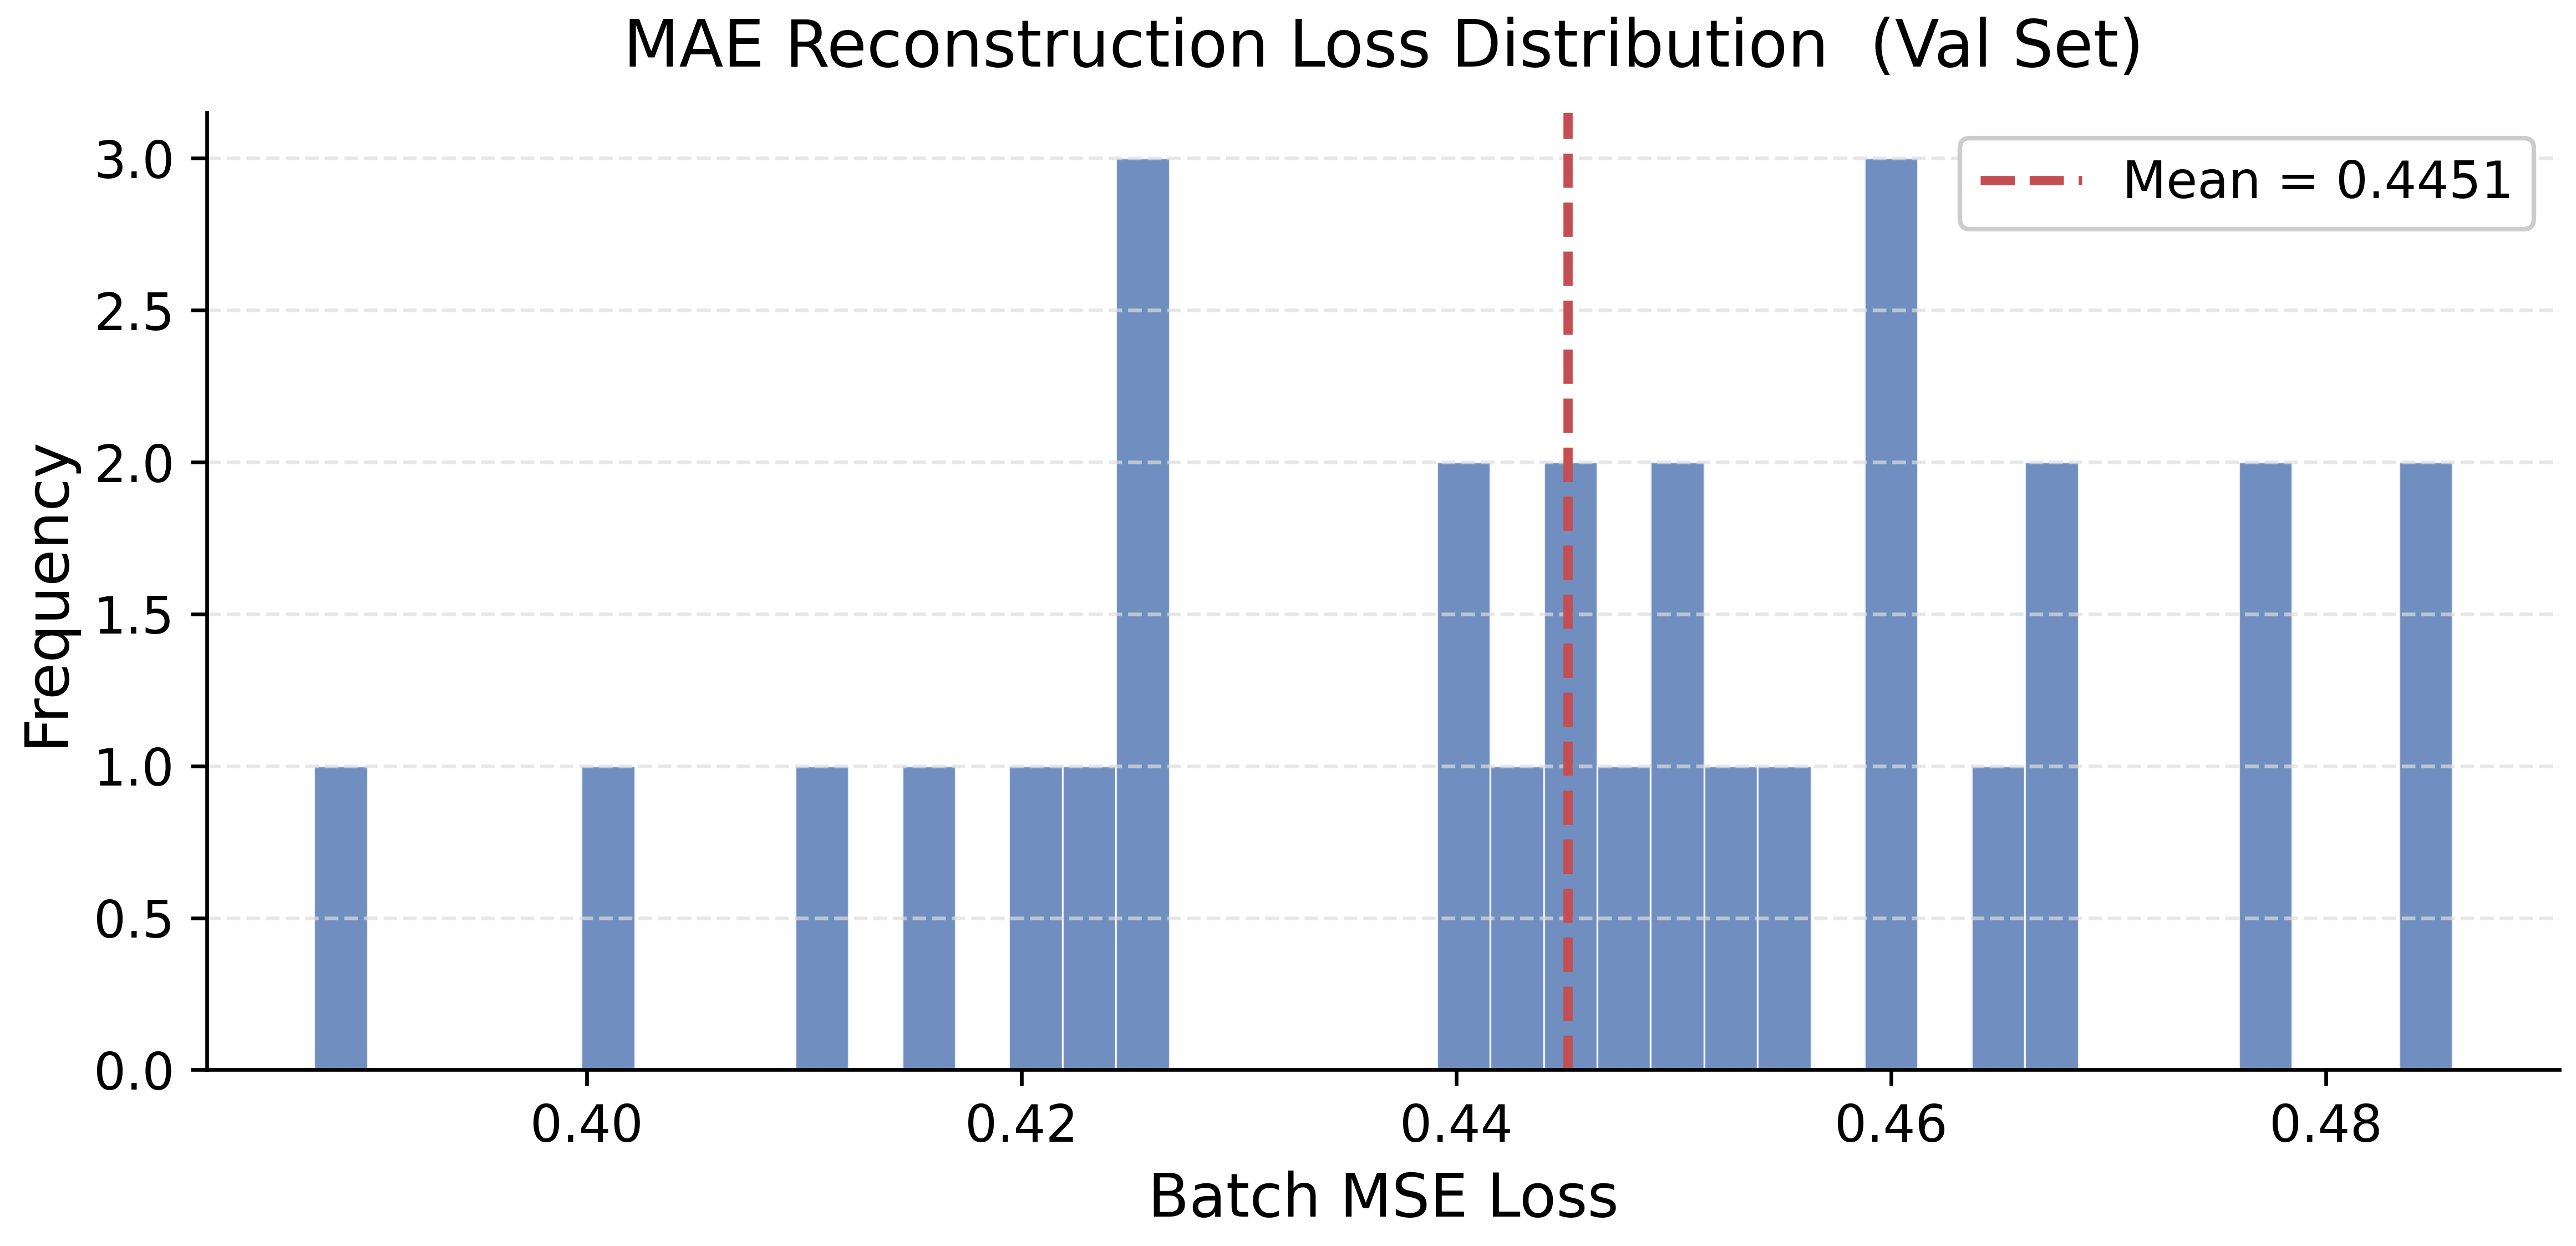
\includegraphics[width=5.5in]{images/mae/01_reconstruction_loss_distribution.png}
\caption{Distribution of per-batch reconstruction MSE loss on the validation set ($n=1{,}801$). Mean $=0.4418$ (dashed line), std $=0.0252$. The narrow symmetric distribution confirms stable MAE convergence.}
\label{fig:recon_loss}
\end{figure*}

\begin{figure*}[!t]
\centering

\includegraphics[width=6.5in]{images/mae/02_reconstruction_grid.png}
\caption{Qualitative MAE reconstruction on 8 validation images. Top: originals. Middle: masked input (75\% patches removed, shown grey). Bottom: decoder reconstruction from 25\% visible patches. The decoder recovers leaf shape, vein structure, and disease lesion locations despite extreme masking.}
\label{fig:recon_grid}
\end{figure*}



\subsubsection{\textit{\textbf{Linear Probe}}}

To assess the quality of the learned representations independently of any supervised fine-tuning, we train a single linear classification head on top of the frozen MAE encoder. The encoder weights are held fixed throughout; no disease labels are used at any point during MAE pretraining. The linear head is trained for 30 epochs on 80\% of the validation split and evaluated on the remaining 20\%. This protocol follows the standard linear evaluation framework for self-supervised representations~\cite{7}. On the test set, the frozen encoder achieves 94.56\% Top-1 accuracy and 100.00\% Top-5 accuracy with a single linear layer. The gap between Top-1 and Top-5 accuracy indicates that the three misclassified-at-Top-1 disease pairs are consistently ranked within the top five predictions, suggesting that even the encoder’s most confusable classes are not represented as outliers in the embedding space. 
As shown in Fig.~\ref{fig:linear_probe}, the linear probe converges rapidly while maintaining a small gap between the training and validation curves.

\begin{figure*}[!t]
\centering
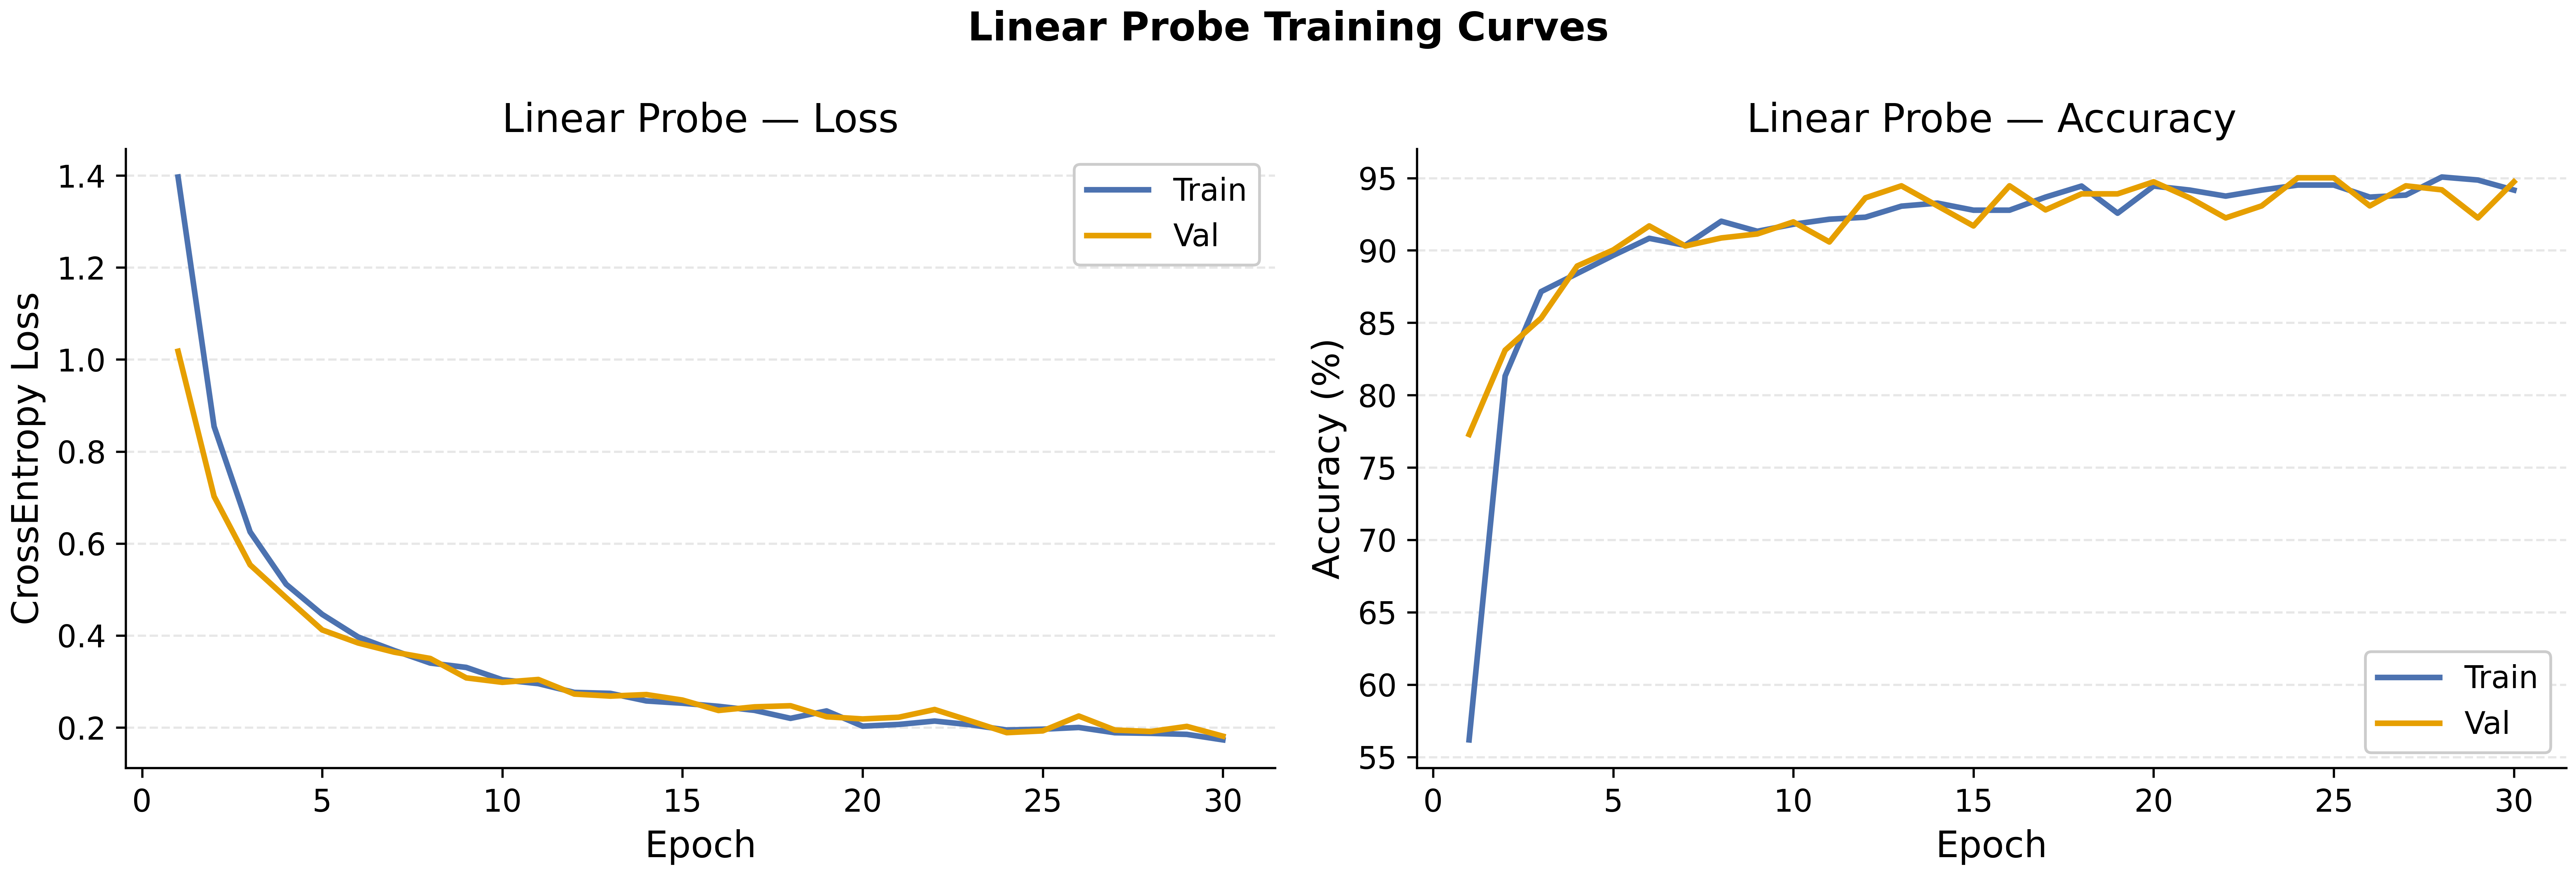
\includegraphics[width=6.5in]{images/mae/03_linear_probe_curves.png}
\caption{Linear probe training curves (30 epochs, frozen MAE encoder). Left: cross-entropy loss. Right: Top-1 accuracy. Train and val curves converge tightly. Best val accuracy: 94.5\%.}
\label{fig:linear_probe}
\end{figure*}



\subsubsection{\textit{\textbf{t-SNE and Cosine Similarity Analysis}}}

Figure~\ref{fig:tsne_mae} shows a t-SNE projection of the frozen encoder embeddings for all 1,802 test images. Three classes---\textit{tomato\_healthy}, \textit{potato\_early}, and \textit{potato\_healthy}---form distinct, well-separated clusters. The remaining three classes---\textit{potato\_late}, \textit{tomato\_late}, and \textit{tomato\_early}---overlap in a central region of the projection. This overlap is consistent with the known visual similarity between late blight presentations on potato and tomato, both caused by \textit{Phytophthora infestans}, which produces morphologically similar lesions across host species. The per-class cosine similarity heatmap (Fig.~\ref{fig:cosine_heatmap}) corroborates this observation: the highest off-diagonal similarity is observed between \textit{potato\_late} and \textit{tomato\_late} ($0.93$), while the lowest is between \textit{tomato\_healthy} and \textit{potato\_early} ($0.79$). We note that interpreting these patterns as definitive evidence of biologically meaningful clustering requires care; the overlap may also reflect limitations in the encoder's ability to distinguish these classes without label supervision, which is addressed in Stage~2.

\begin{figure*}[!t]
\centering
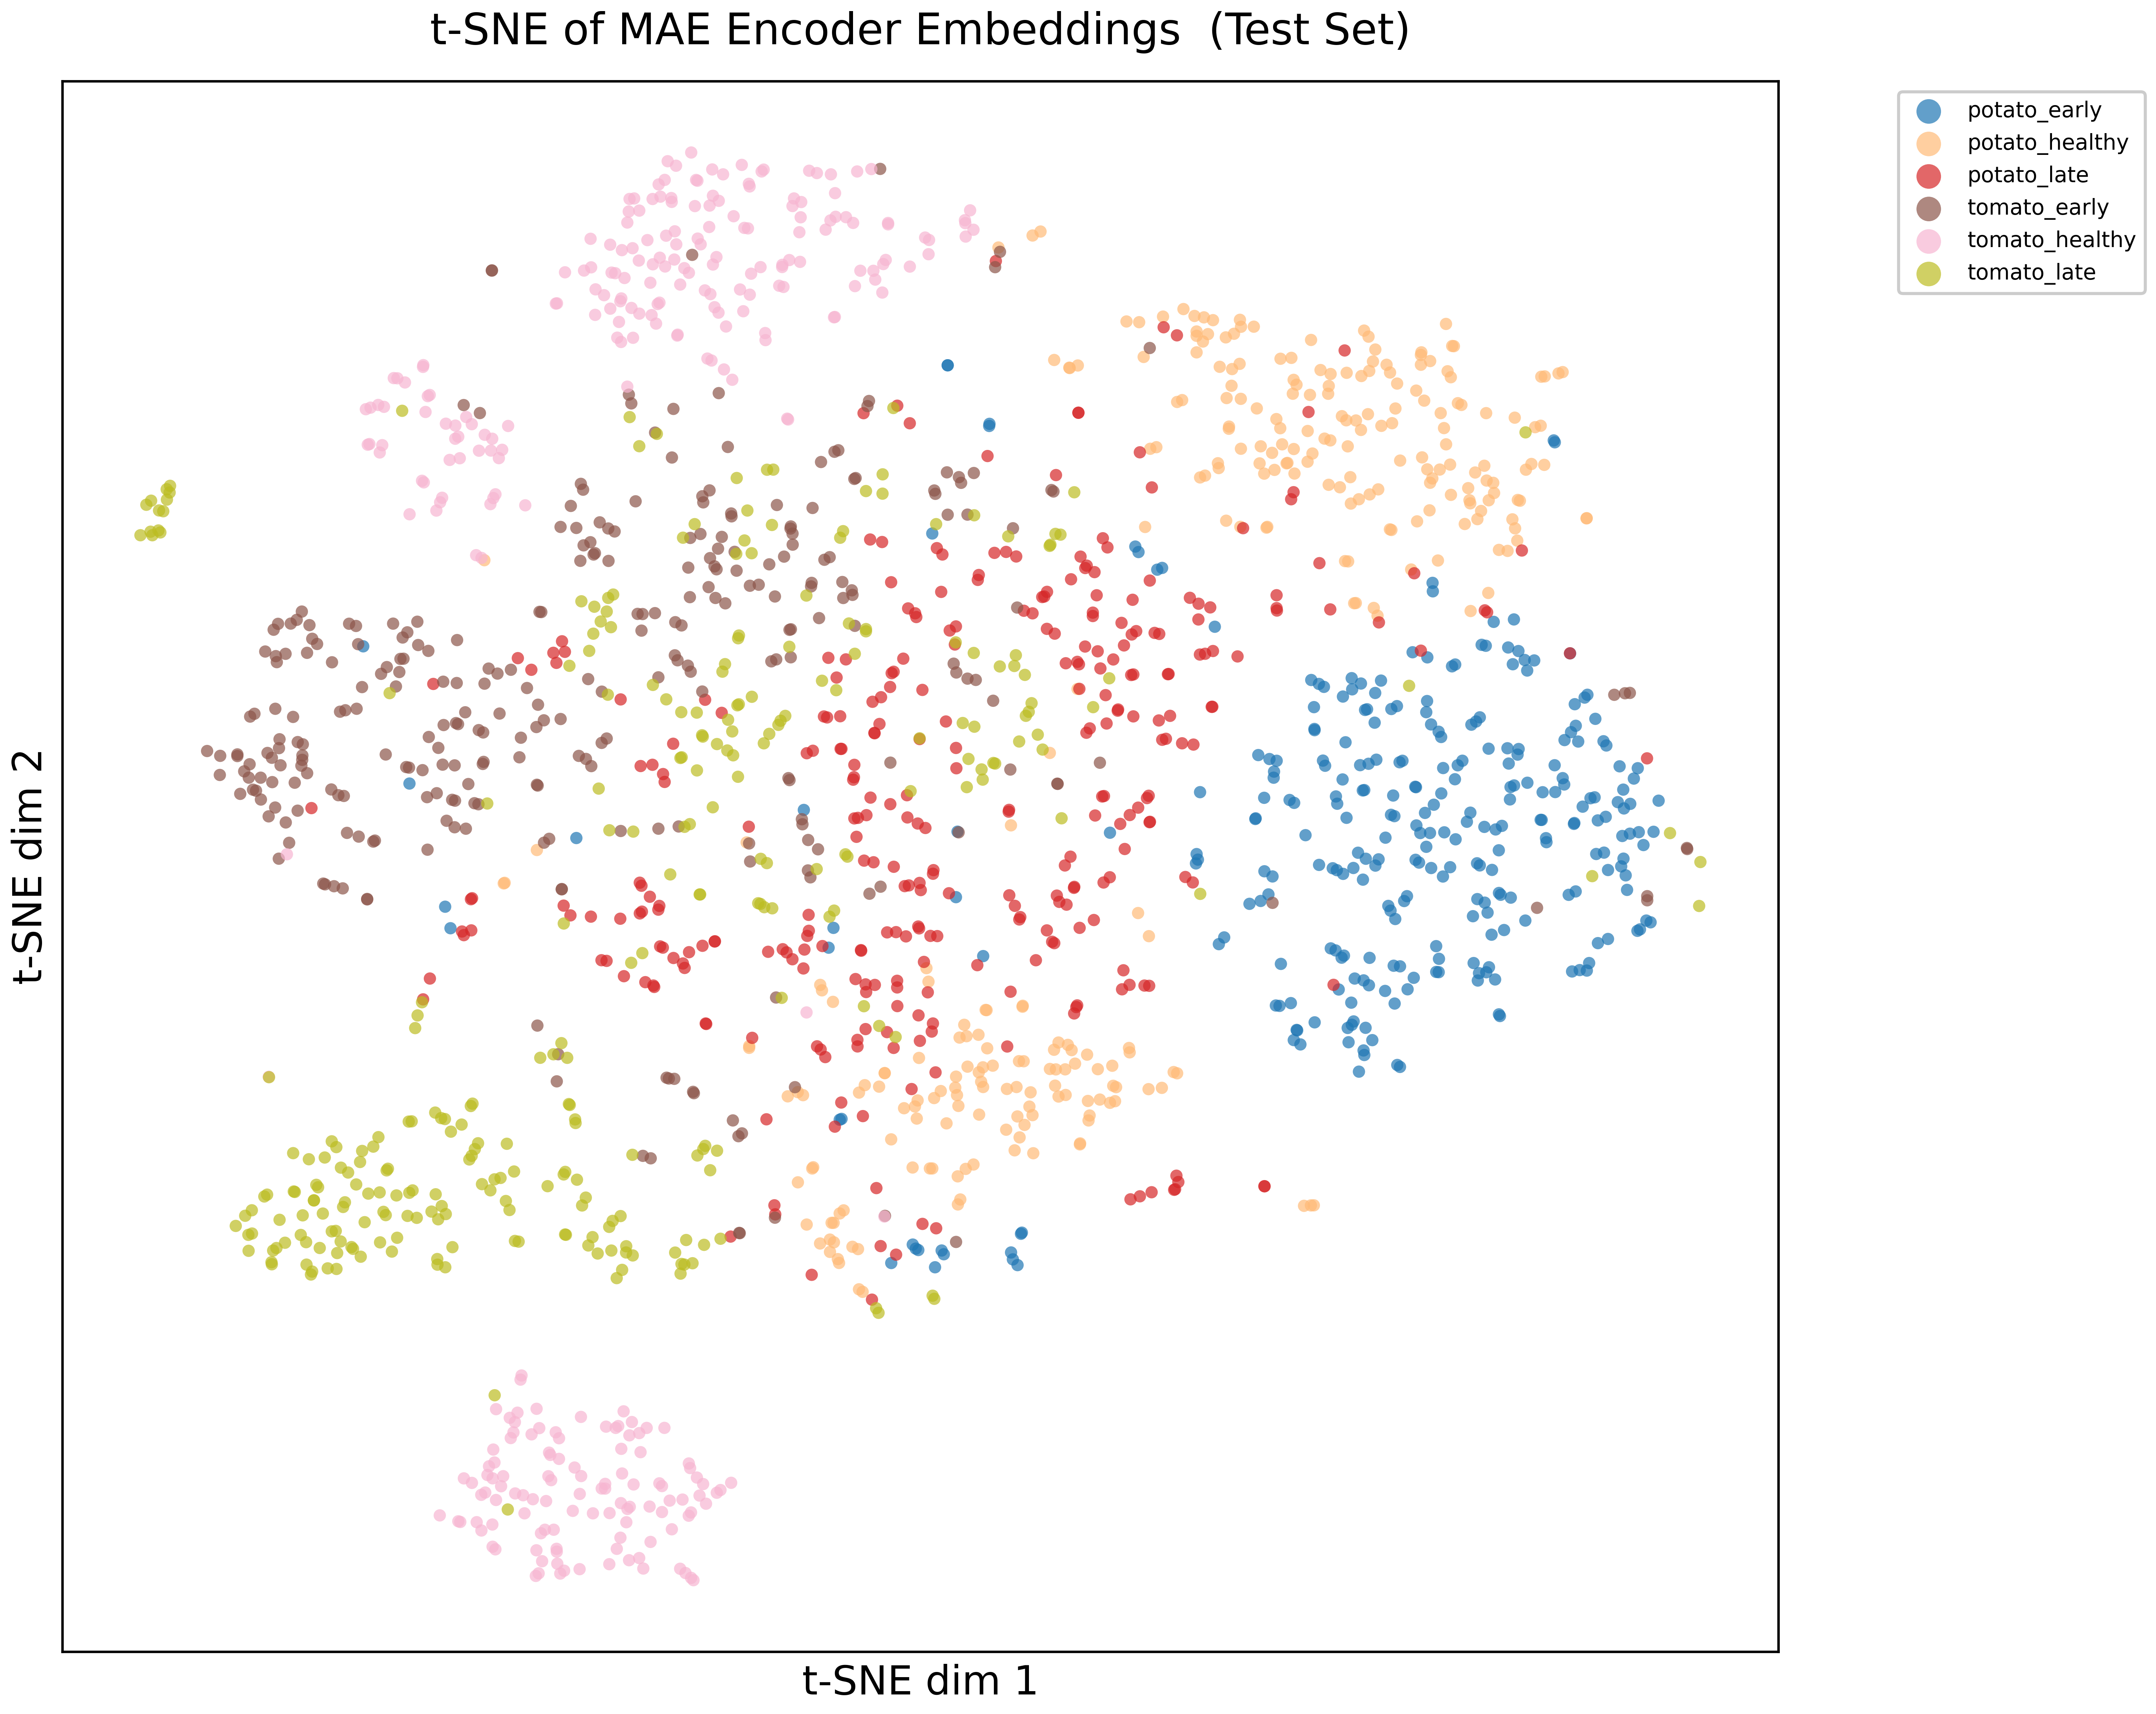
\includegraphics[width=5.5in]{images/mae/08_tsne_embeddings.png}
\caption{t-SNE of frozen MAE encoder embeddings (test set, 1,802 points). Three classes form clean isolated clusters (\textit{tomato\_healthy}, \textit{potato\_early}, \textit{potato\_healthy}). Central overlap between \textit{potato\_late}, \textit{tomato\_late}, and \textit{tomato\_early} reflects their biological similarity---late blight on both crops is caused by the same pathogen (\textit{Phytophthora infestans}). This overlap is fully resolved by CLViT fine-tuning (see Fig.~\ref{fig:tsne_clvit_class}).}
\label{fig:tsne_mae}
\end{figure*}

\begin{figure*}[!t]
\centering
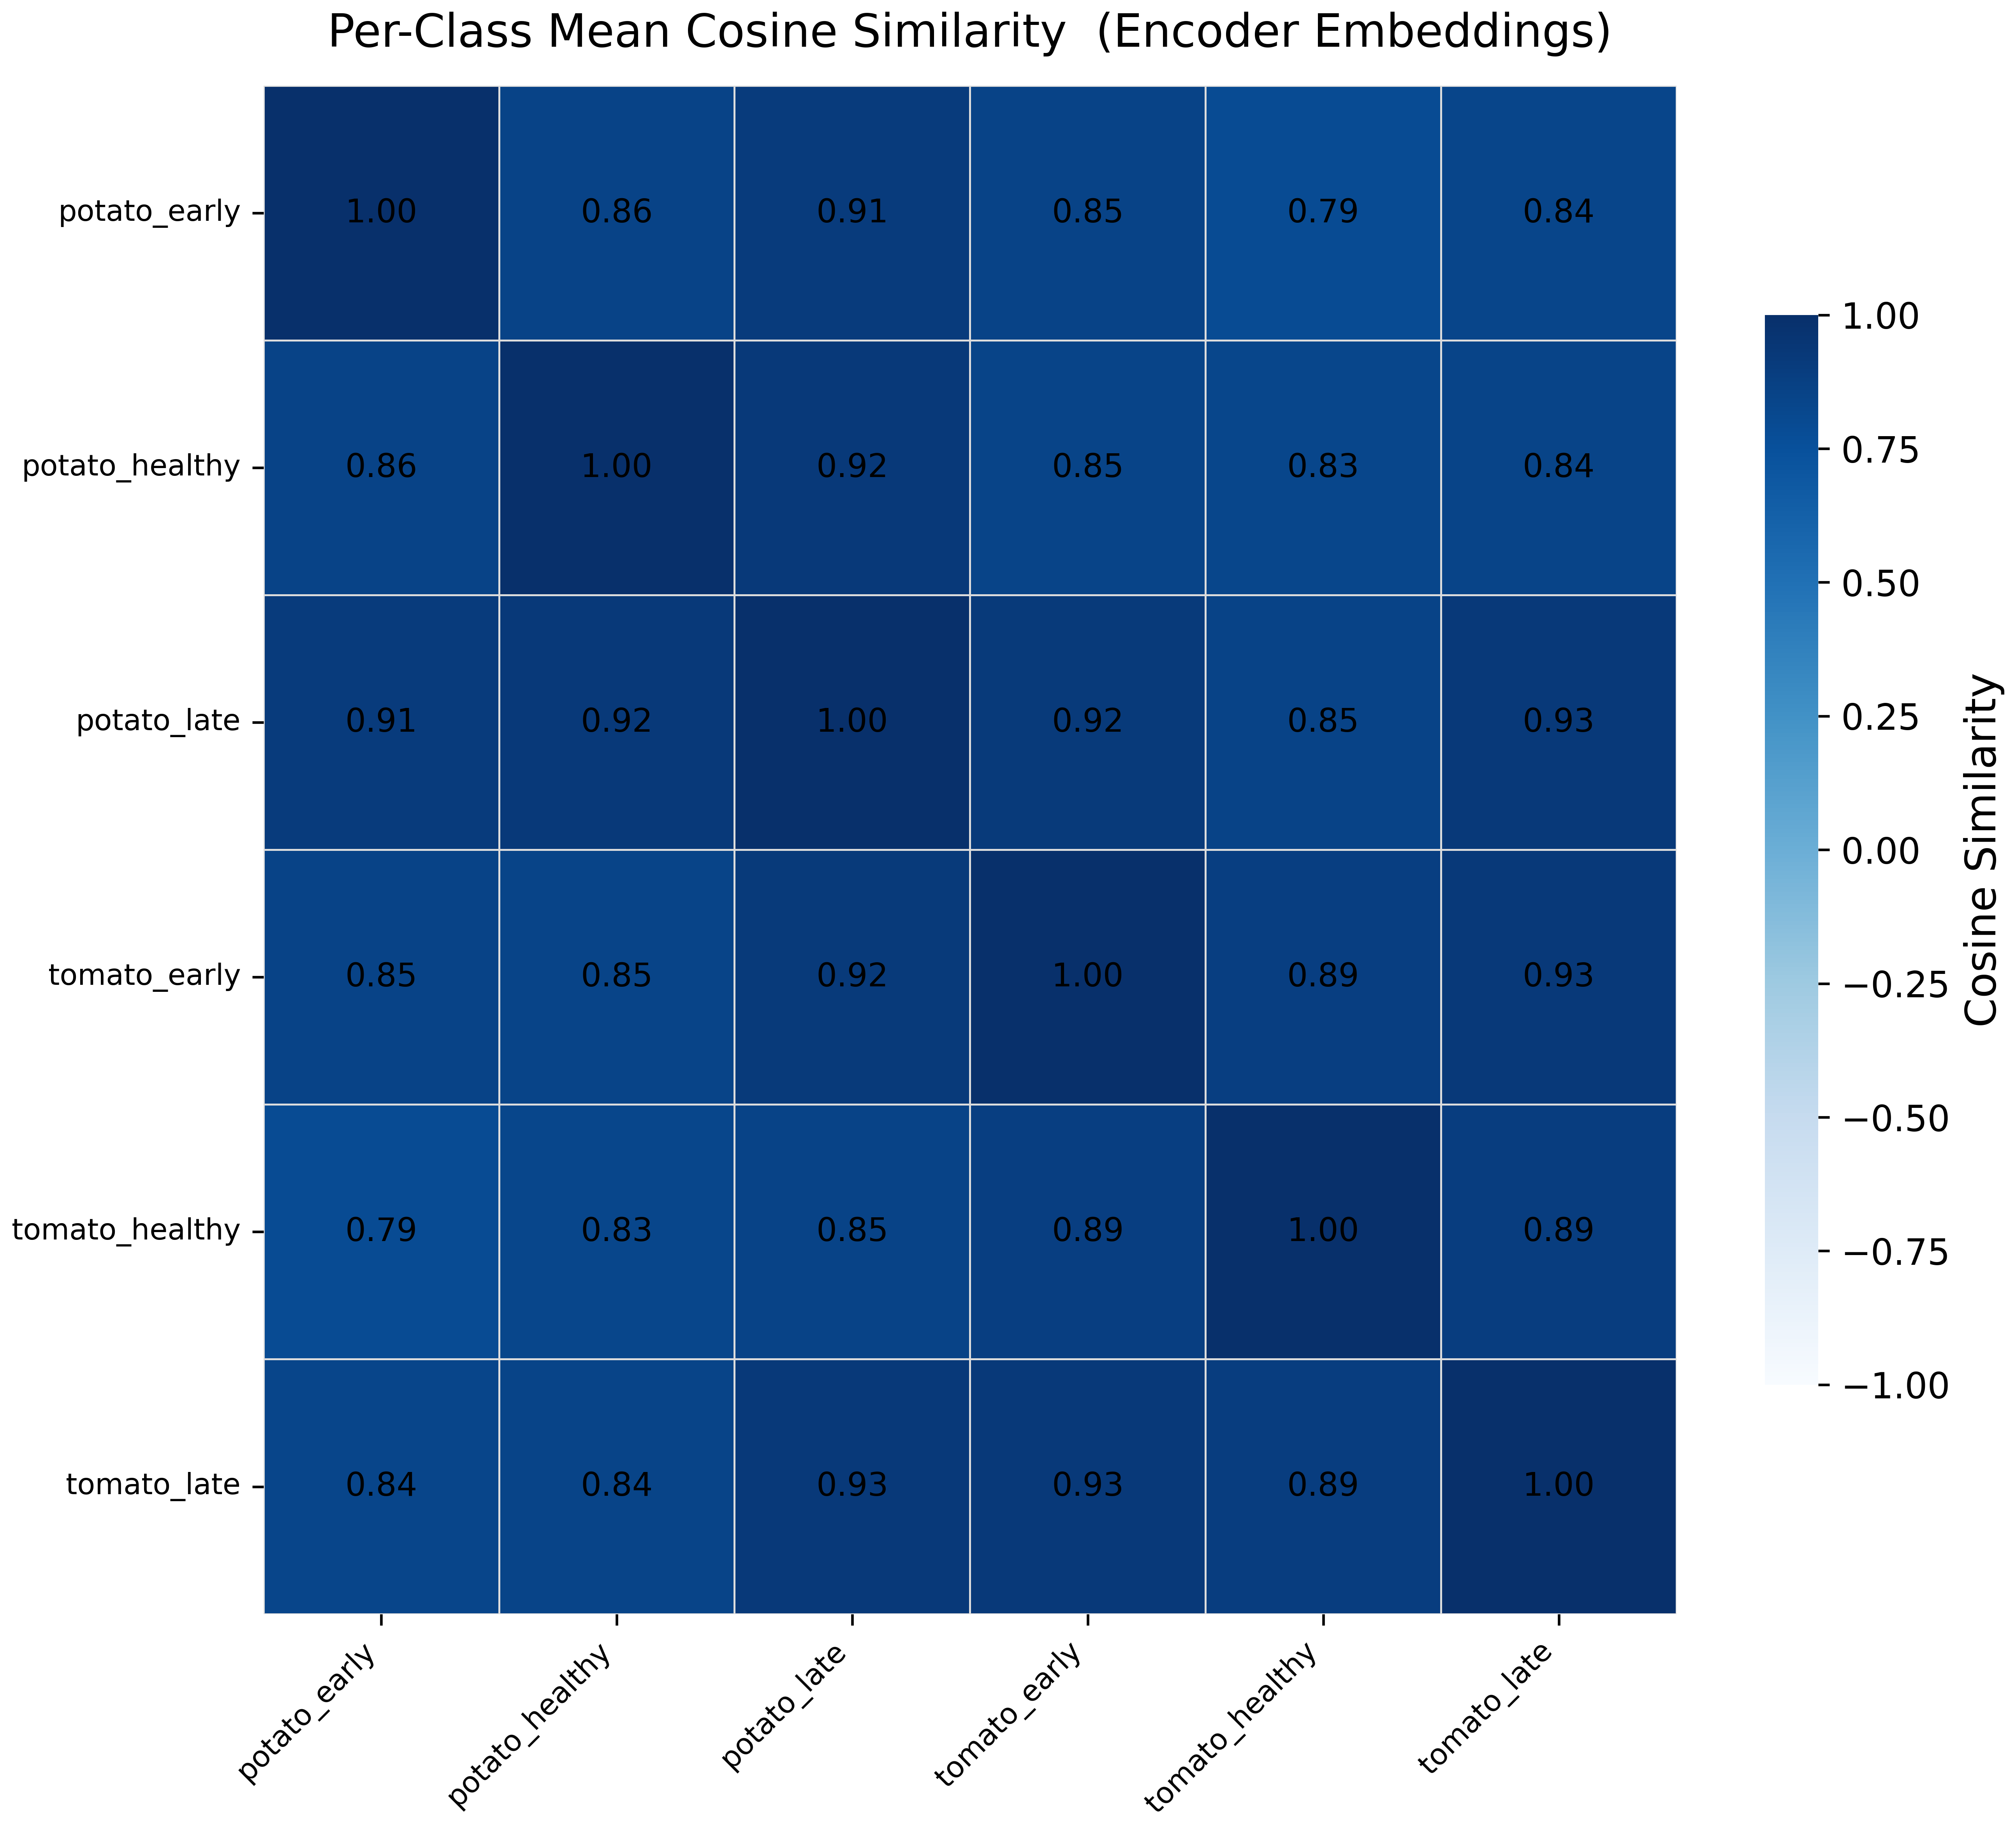
\includegraphics[width=5.0in]{images/mae/09_cosine_similarity_heatmap.png}
\caption{Cosine similarity between per-class mean MAE encoder embeddings. Highest off-diagonal: \textit{potato\_late} vs \textit{tomato\_late} (0.93), biologically explained by shared \textit{P. infestans} pathogen. Lowest off-diagonal: \textit{tomato\_healthy} vs \textit{potato\_early} (0.79). All values in $[0.79, 1.00]$.}
\label{fig:cosine_heatmap}
\end{figure*}



\subsection{CLViT Performance}

CLViT is trained for 100 epochs with differential learning rates (encoder: $3\times10^{-5}$; new modules: $3\times10^{-4}$) and a 5-epoch cosine warmup schedule. Validation accuracy is monitored after each epoch, and the best checkpoint is retained. CLViT first exceeds the frozen linear probe baseline (94.56\%) at epoch~2 and reaches 99.50\% validation accuracy at epoch~21. The best validation accuracy of 99.89\% is achieved at epoch~84.

The supervised classification loss ($L_{\mathrm{sup}}$) decreases monotonically from 1.046 at epoch~1 to 0.461 at epoch~100, indicating continued learning throughout training. The auxiliary rotation loss decreases from 1.416 (chance level: $\ln(4)\approx1.386$) to 0.404, confirming that the rotation prediction head learns informative geometric features rather than converging to chance. The flip loss stabilises at approximately 0.52, close to the chance level for a binary task ($\ln(2)\approx0.693$), which is consistent with the symmetric appearance of leaf images under horizontal reflection and indicates that flip prediction contributes primarily as a weak regulariser rather than a strong self-supervised signal in this domain.

We note that all validation accuracy figures reported in this subsection are measured on the validation split ($n=1,801$) and are distinct from the test set results reported in Section~5.B.

As shown in Fig.~\ref{fig:cosine_heatmap}, the cosine similarity heatmap corroborates the clustering observed in the t-SNE projection.

As shown in Fig.~\ref{fig:clvit_dashboard}, CLViT achieves consistently high performance across multiple evaluation metrics while exhibiting reduced robustness under severe brightness perturbations.

\begin{figure*}[!t]
\centering

\includegraphics[width=6.5in]{images/clvit/00_summary_dashboard.png}
\caption{CLViT test-set evaluation summary. Top-1: 99.83\%. Macro F1: 99.83\%. AUC-OvR: 99.99\%. MCC: 99.80\%. ECE: 6.60\%. Worst robustness drop: $-44.2\%$ (brightness $-40\%$).}
\label{fig:clvit_dashboard}
\end{figure*}



\begin{table}[H]
\centering
\caption{\textit{CLViT Test Performance}}
\label{tab:clvit_metrics}
\begin{tabular}{lc}
\toprule
Metric & Value\\
\midrule
Top-1 Accuracy & 99.83\%\\
Top-3 Accuracy & 100.00\%\\
Top-5 Accuracy & 100.00\%\\
Macro F1 & 99.83\%\\
Weighted F1 & 99.83\%\\
AUC-OvR & 99.99\%\\
MCC & 99.80\%\\
ECE & 6.60\%\\
\bottomrule
\end{tabular}
\end{table}

\begin{table}[!t]
\centering
\caption{\textit{Per-class precision, recall, and F1-score on the test set.}}
\label{tab:per_class_metrics}
\begin{tabular}{lcccc}
\toprule
\textbf{Class} & \textbf{Precision} & \textbf{Recall} & \textbf{F1} & \textbf{Support} \\
\midrule
potato\_early    & 1.00 & 1.00 & 1.00 & 289 \\
potato\_healthy  & 1.00 & 1.00 & 1.00 & 298 \\
potato\_late     & 1.00 & 1.00 & 1.00 & 318 \\
tomato\_early    & 1.00 & 0.99 & 1.00 & 301 \\
tomato\_healthy  & 1.00 & 1.00 & 1.00 & 298 \\
tomato\_late     & 0.99 & 1.00 & 0.99 & 298 \\
\midrule
\textbf{Macro Average} & \textbf{1.00} & \textbf{1.00} & \textbf{0.998} & \textbf{1,802} \\
\bottomrule
\end{tabular}
\end{table}



As shown in Fig.~\ref{fig:confusion_raw}, the raw confusion matrix demonstrates that only three misclassifications occur across the entire test set.

\begin{figure*}[!t]
\centering
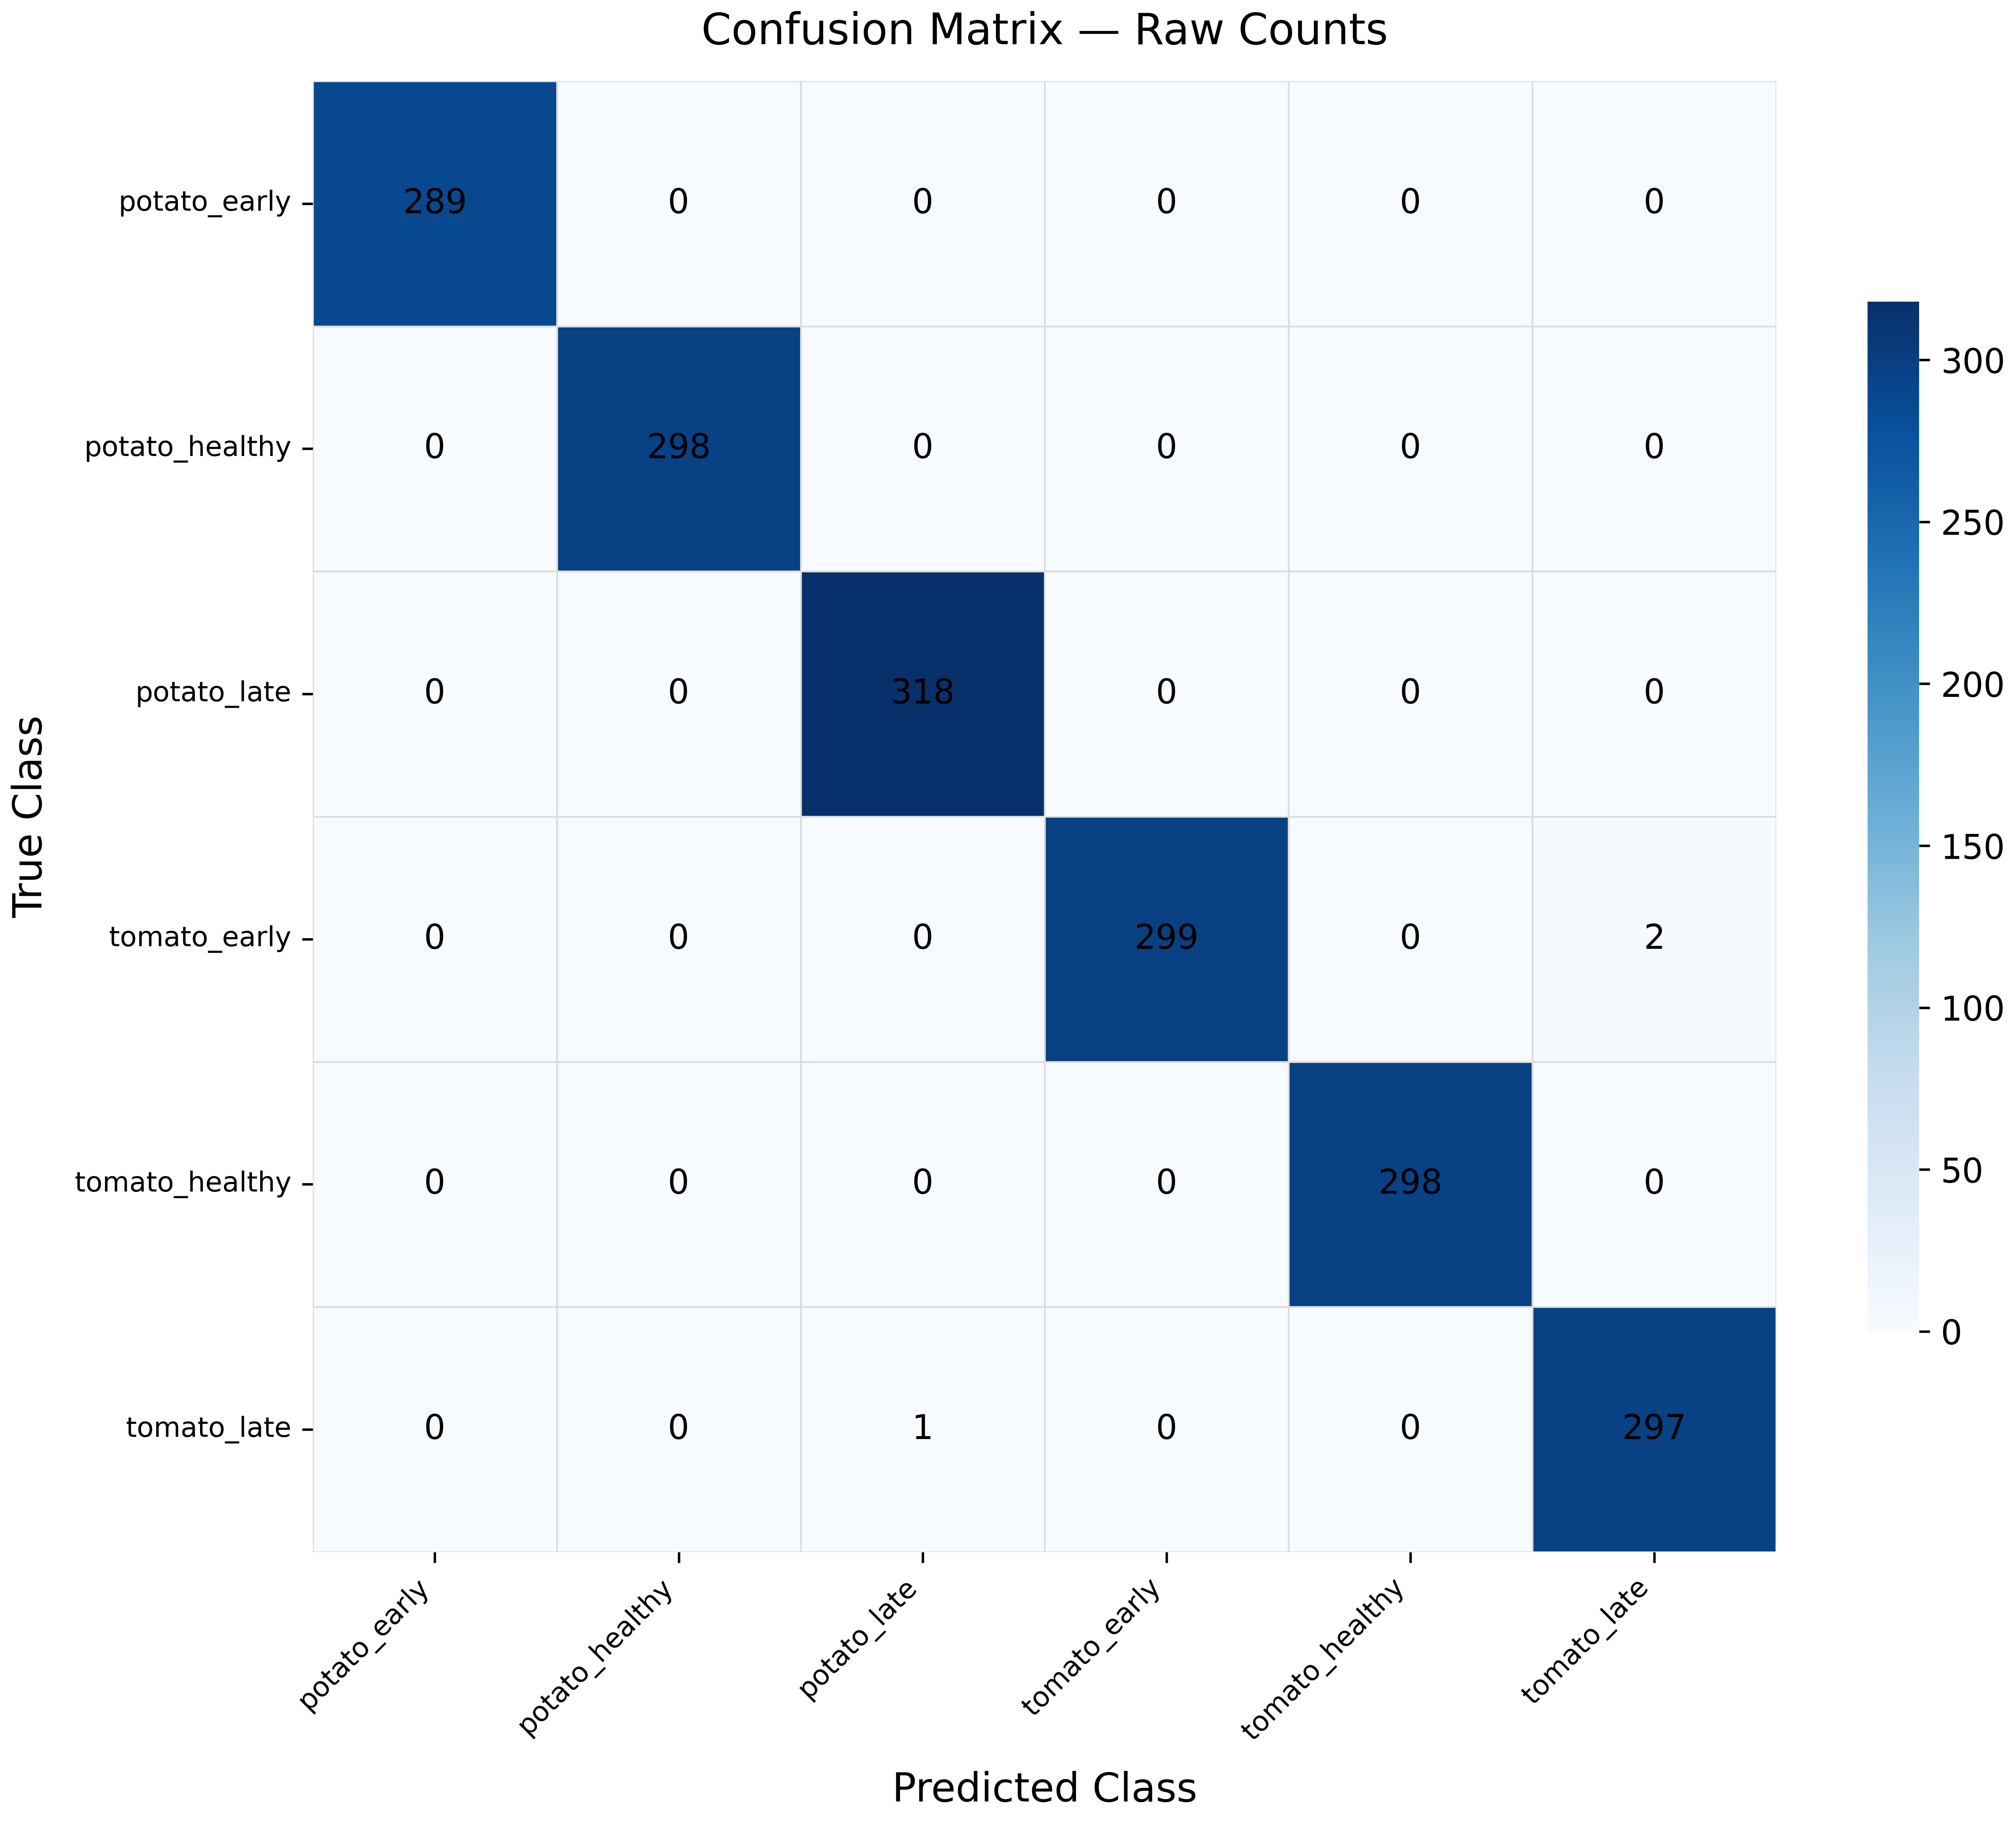
\includegraphics[width=4.5in]{images/clvit/02_confusion_matrix_raw.png}
\caption{Raw confusion matrix on the test set ($n=1{,}802$). Only 3 off-diagonal entries: 2 \textit{tomato\_early} misclassified as \textit{tomato\_late}, 1 \textit{tomato\_late} misclassified as \textit{potato\_late}. All errors are within the biologically similar late blight family.}
\label{fig:confusion_raw}
\end{figure*}

\begin{figure*}[!t]
\centering
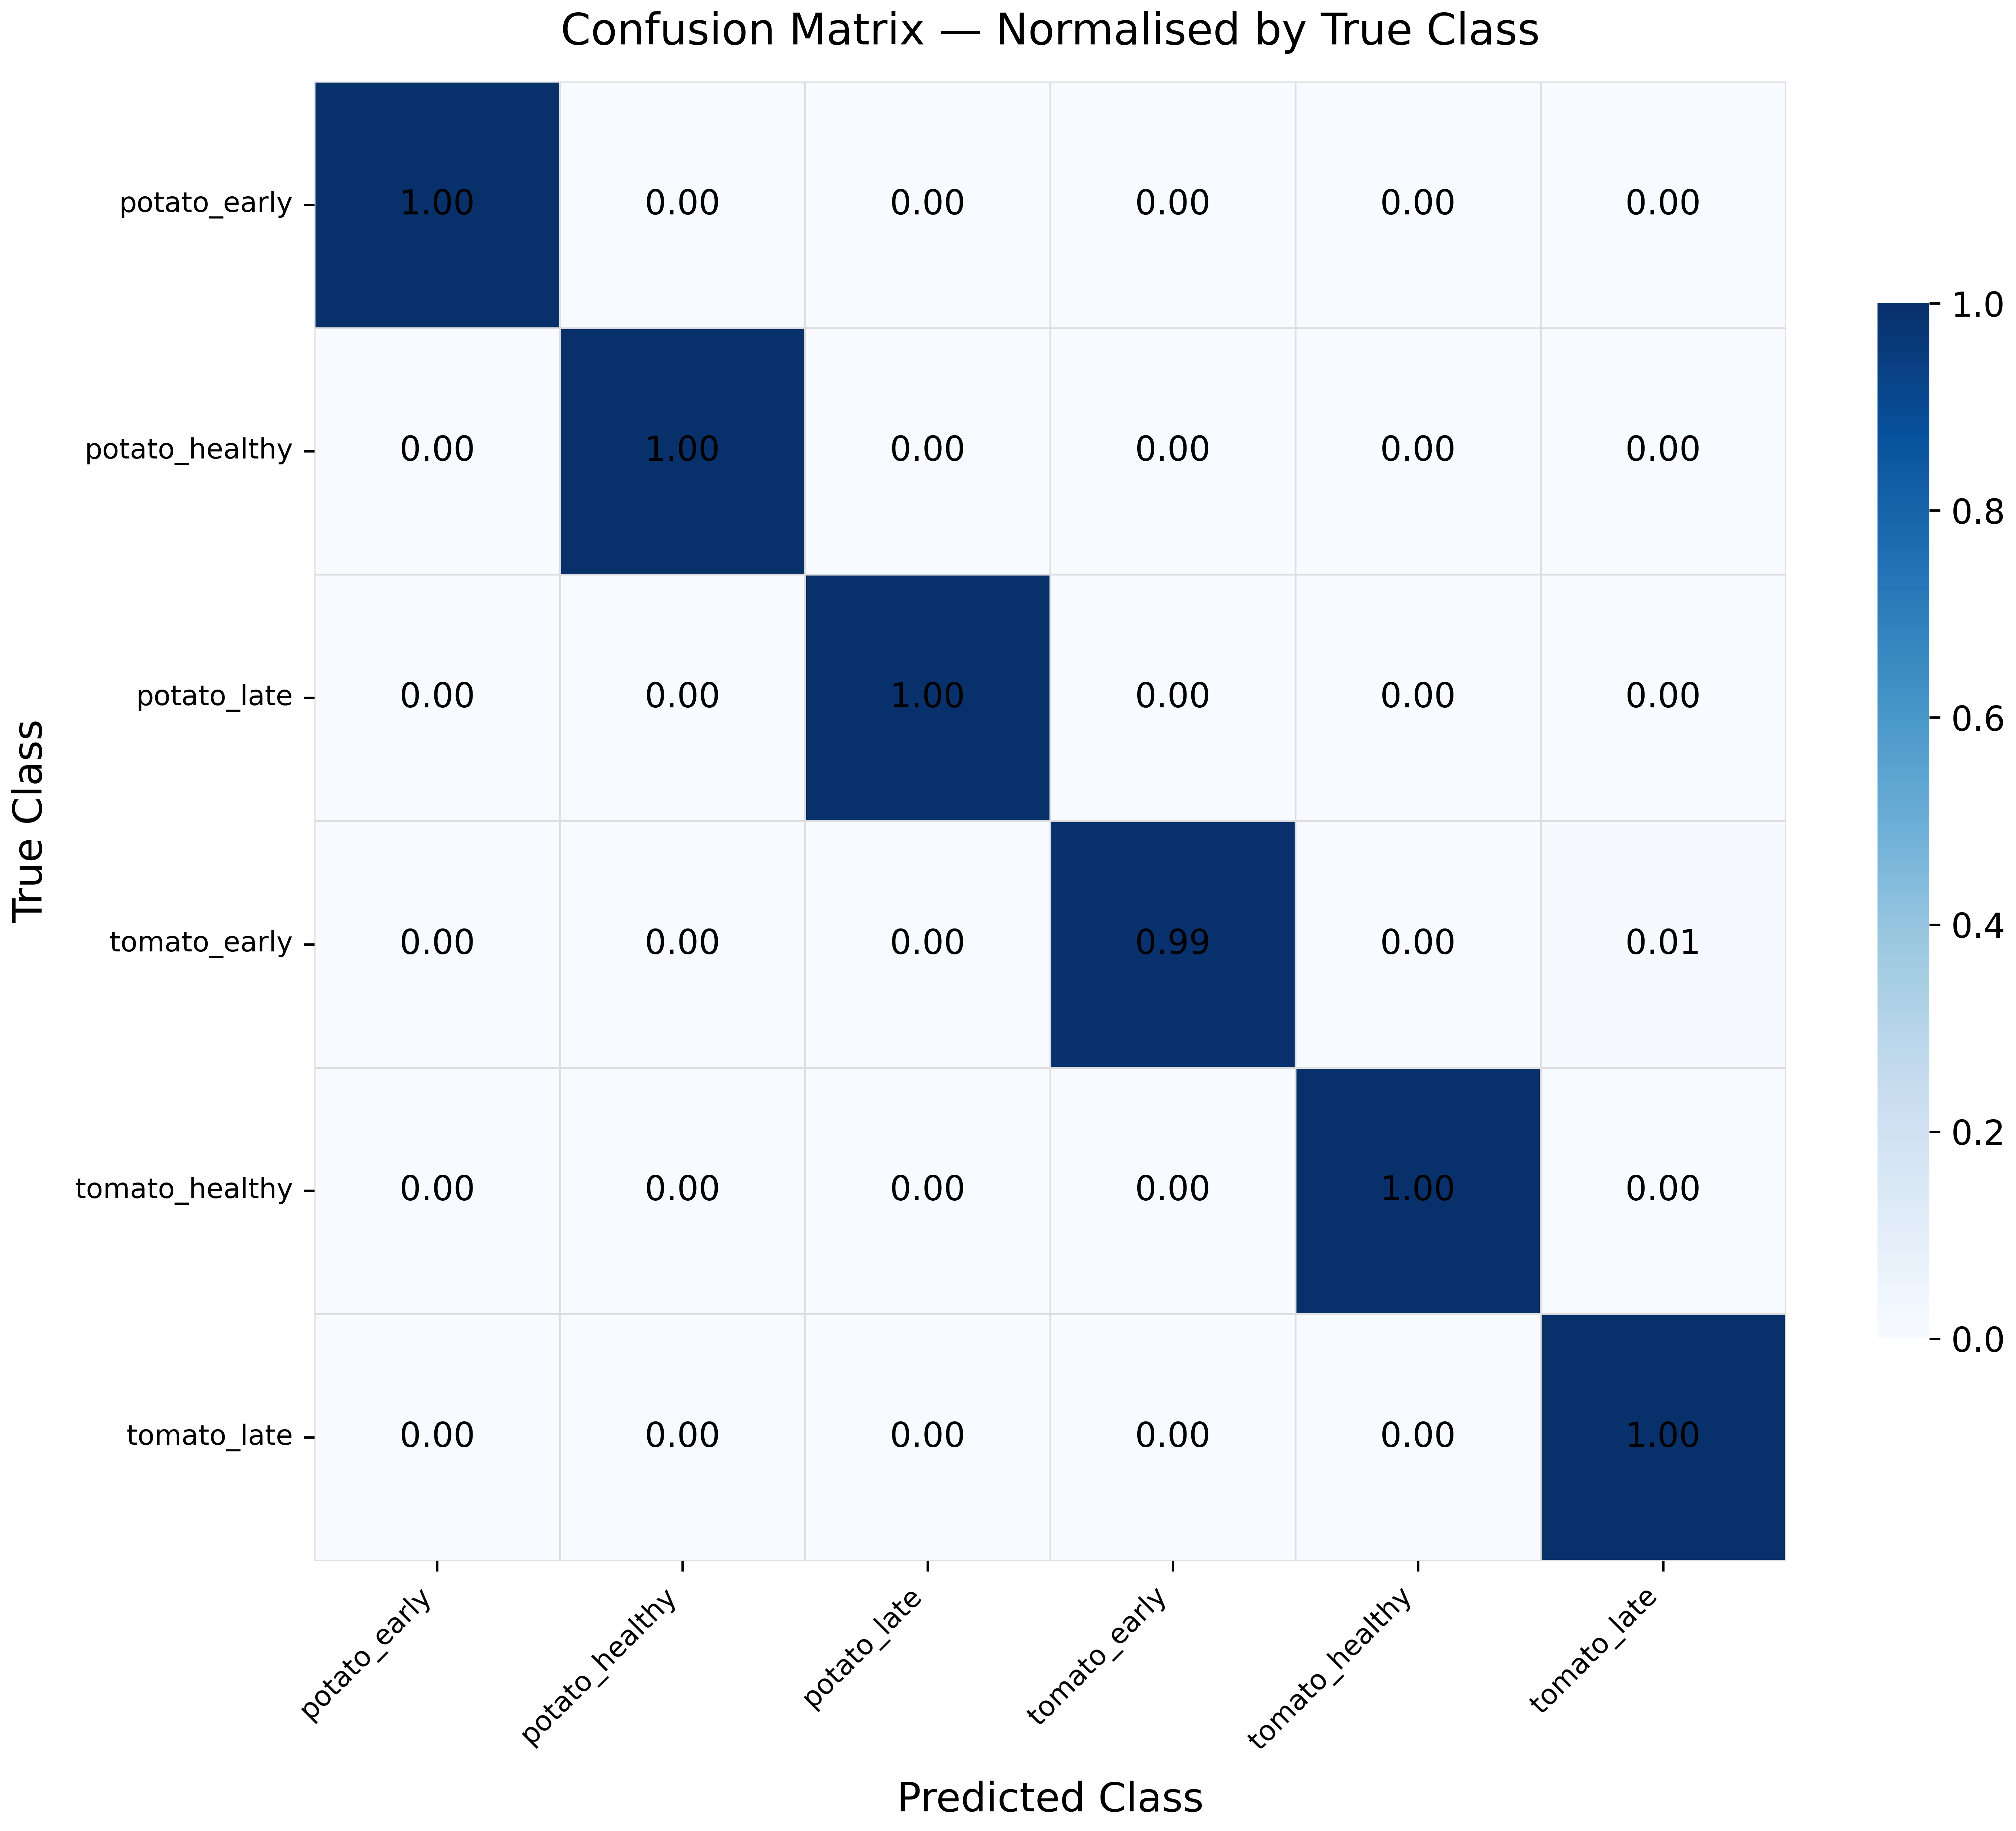
\includegraphics[width=4.5in]{images/clvit/03_confusion_matrix_normalised.png}
\caption{Row-normalised confusion matrix. Five of six classes achieve recall $=1.00$. \textit{tomato\_early} recall $=0.99$ (2 of 301 misclassified). All off-diagonal values are $0.00$ or $0.01$.}
\label{fig:confusion_norm}
\end{figure*}

\begin{figure}[H]
\centering
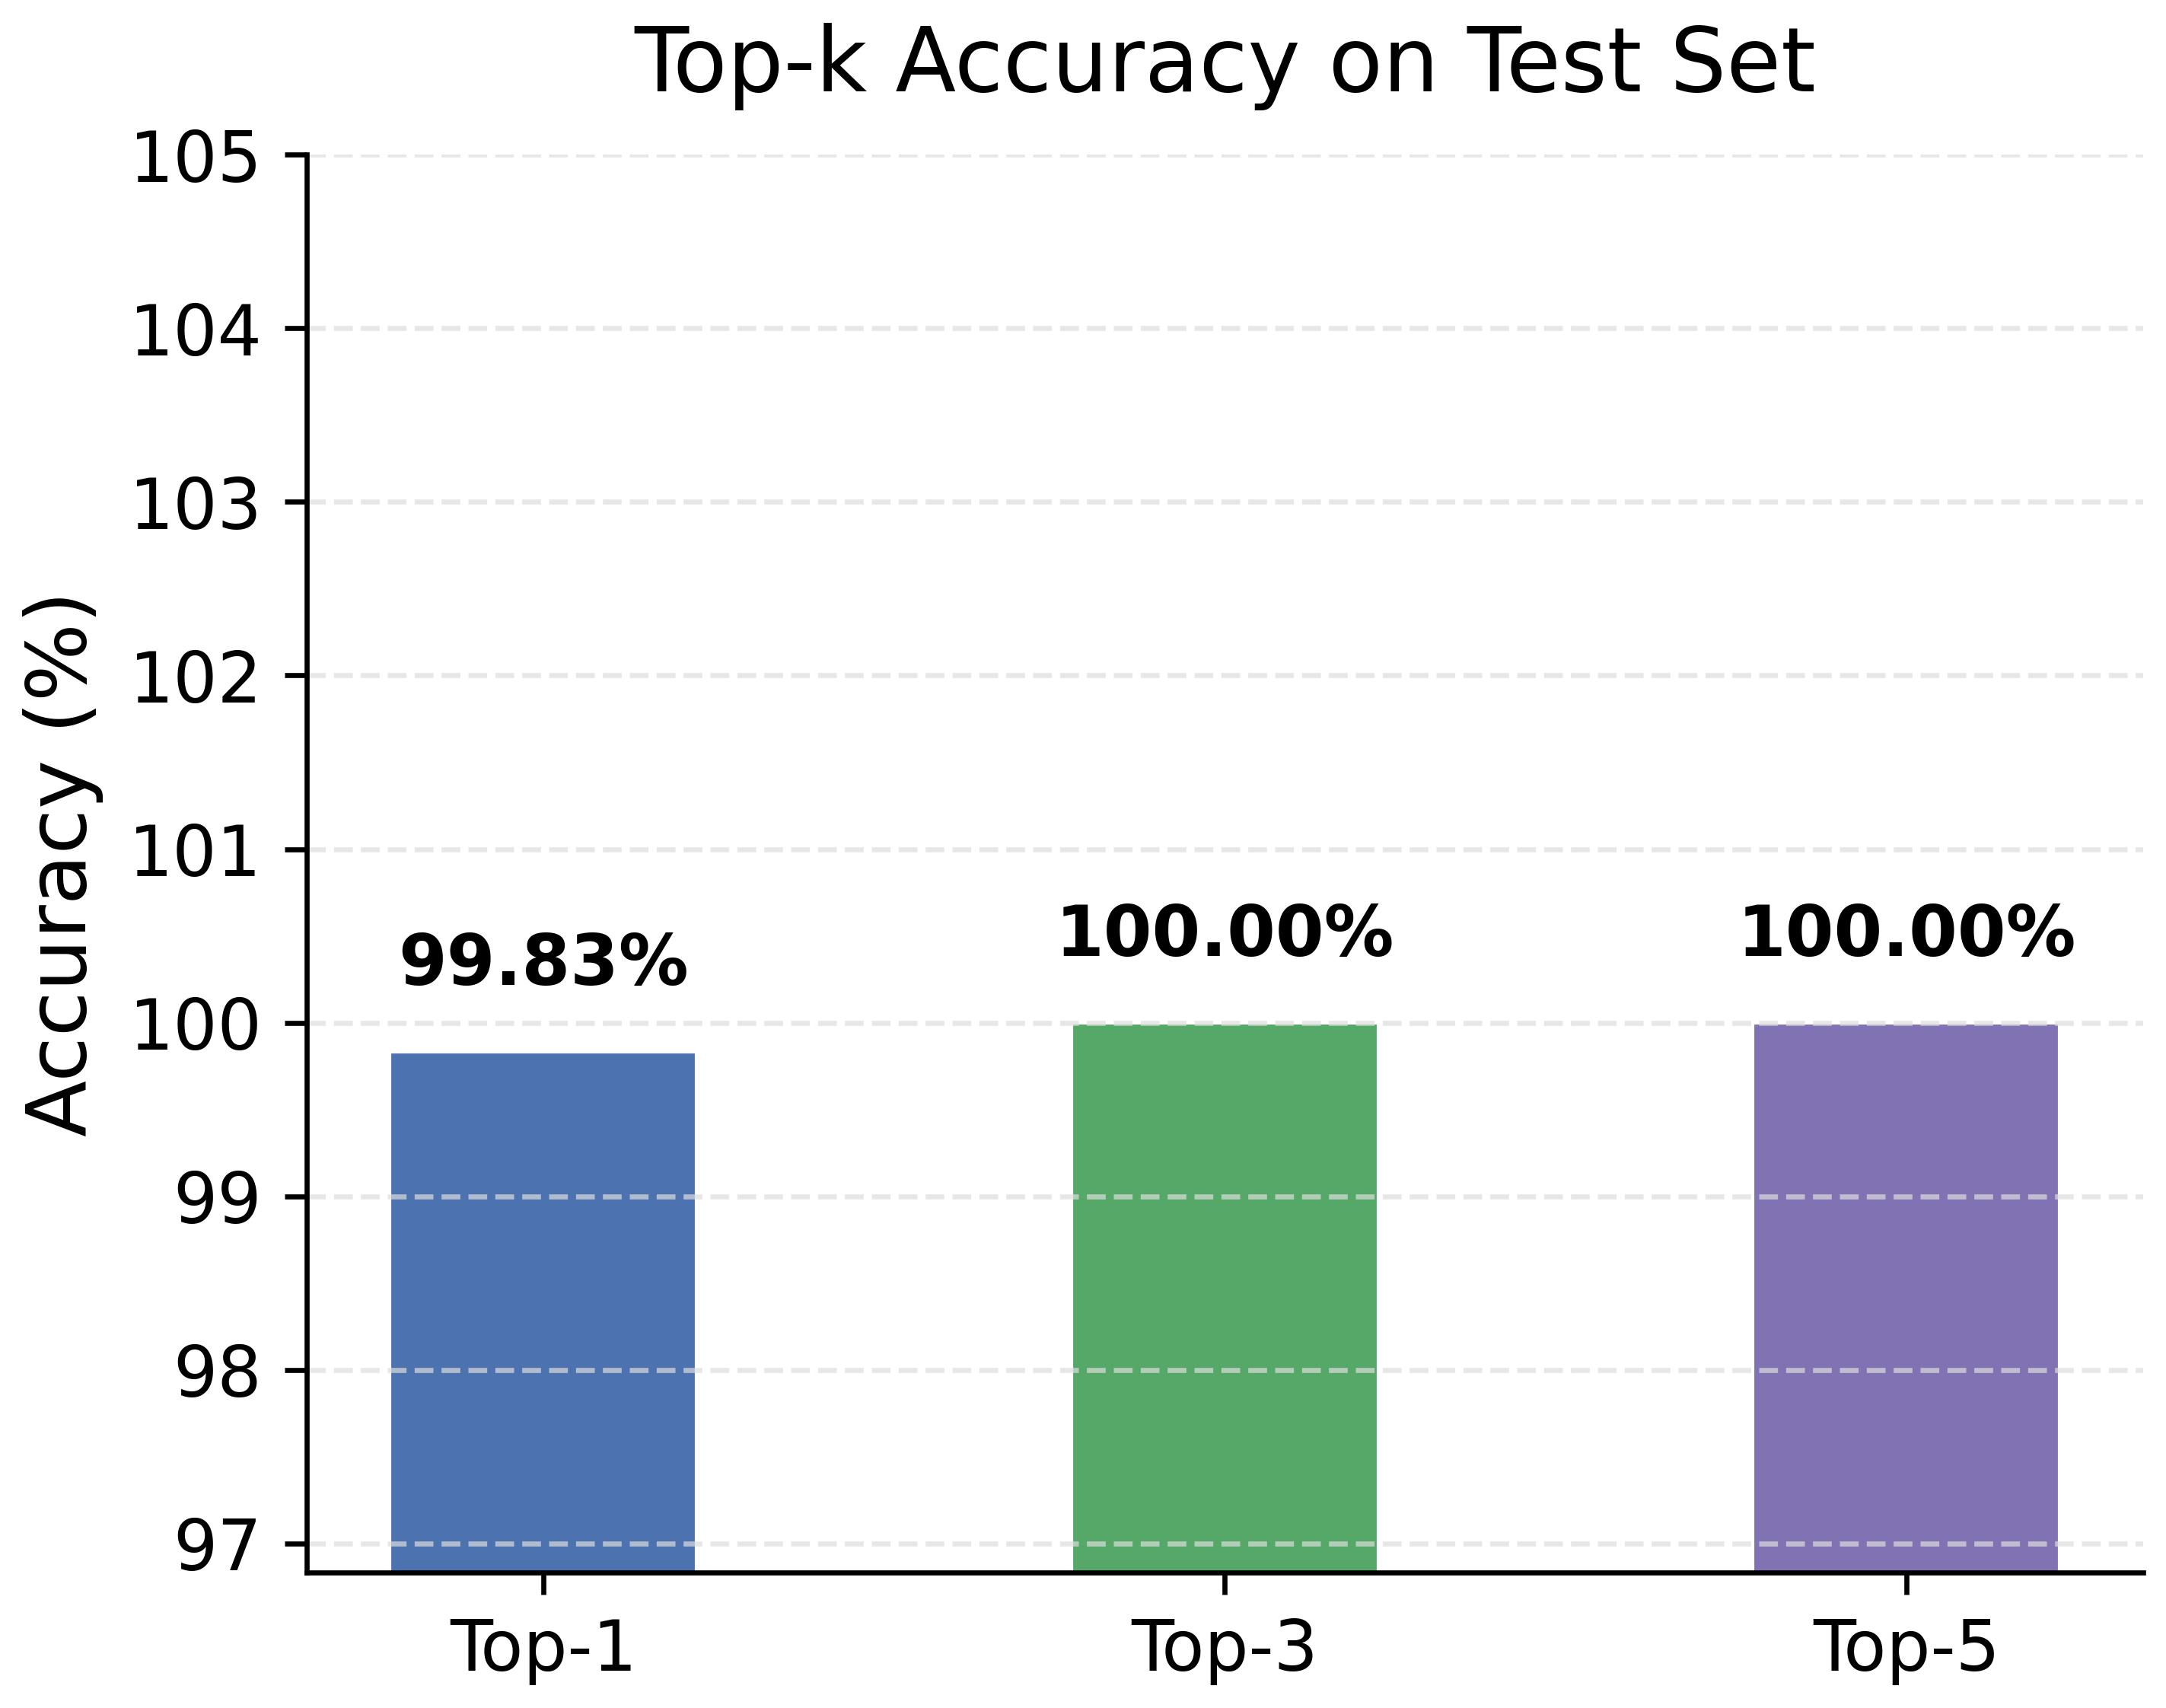
\includegraphics[width=3.3in]{images/clvit/01_topk_accuracy.png}
\caption{Top-1 (99.83\%), Top-3 (100.00\%), and Top-5 (100.00\%) accuracy on the test set. Perfect Top-3/5 accuracy means the correct class is always within the model's top 3 predictions.}
\label{fig:topk}
\end{figure}

\begin{figure*}[!t]
\centering
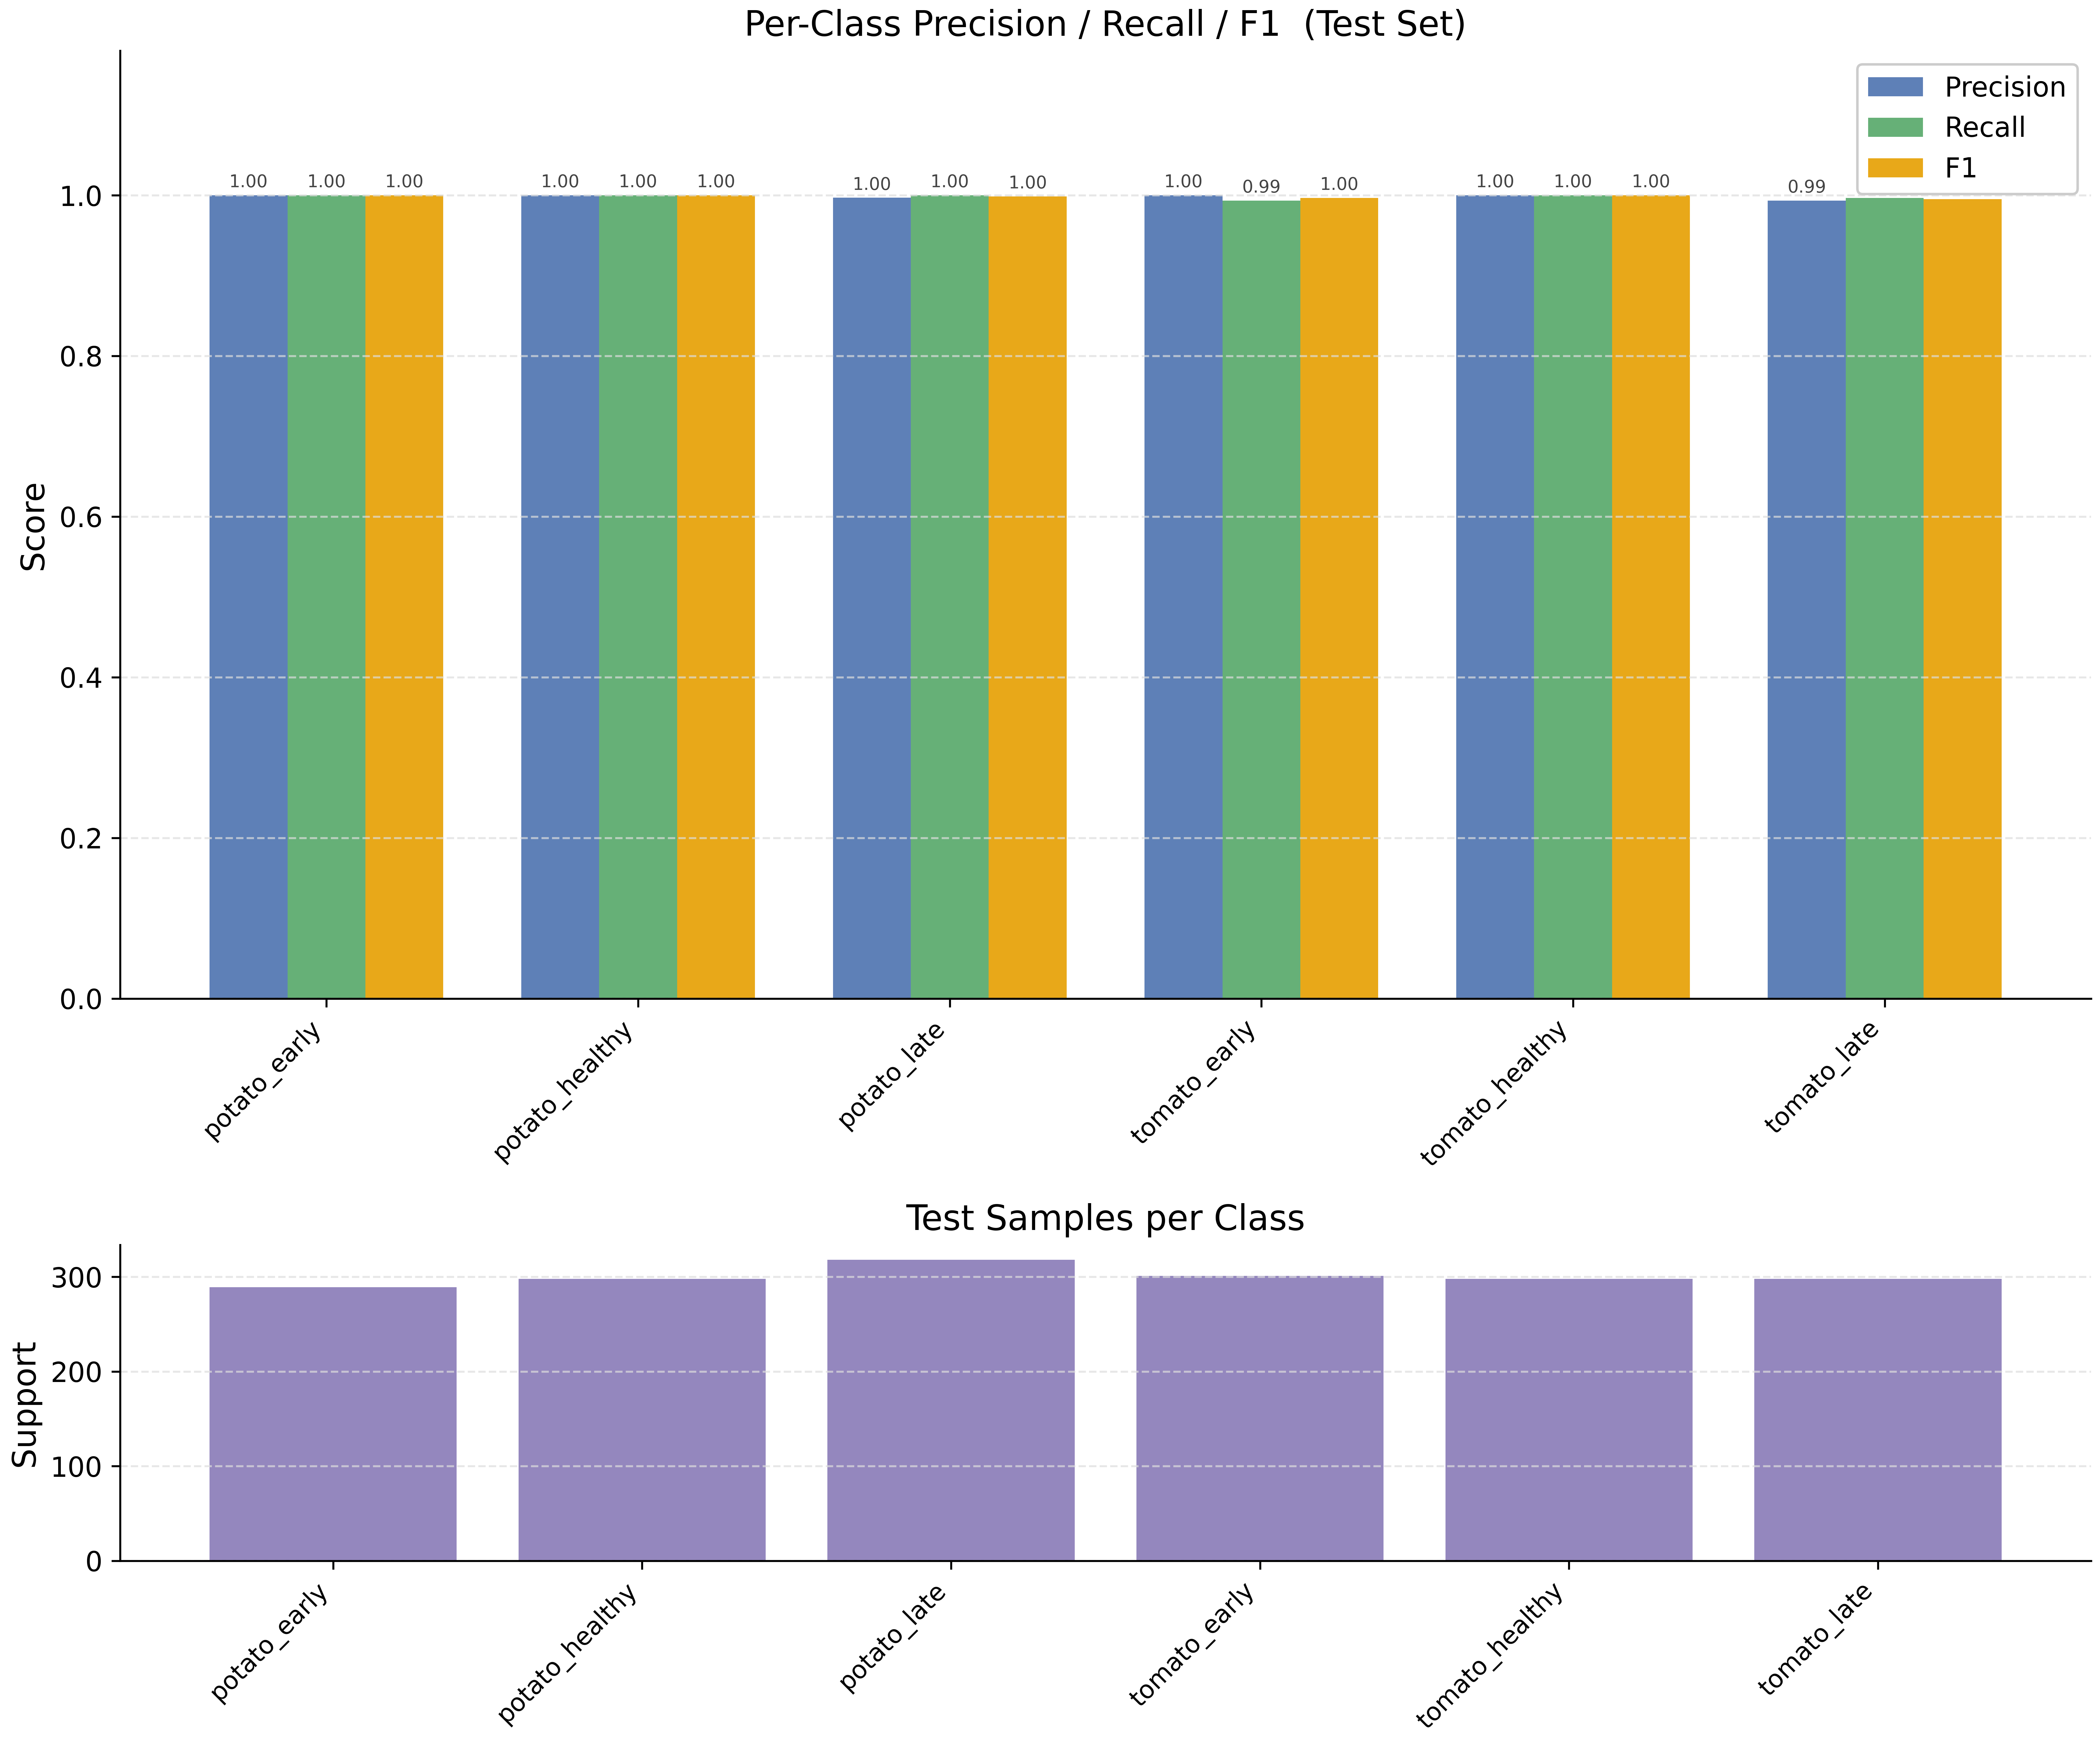
\includegraphics[width=6.5in]{images/clvit/04_per_class_metrics.png}
\caption{Per-class precision, recall, and F1 bar chart (top) with test support counts per class (bottom). All six classes achieve $\geq0.99$ on all three metrics.}
\label{fig:per_class_prf}
\end{figure*}

\subsection{Label Efficiency}

To assess the label efficiency of the proposed pipeline relative to a strong supervised baseline, both CLViT and a ViT-B/16 fine-tuned from ImageNet-21k weights (Section~4.2) are trained independently at four label fractions: 10\%, 25\%, 50\%, and 100\% of the training indices defined by the fixed data split. At each fraction, both models are trained for 50 epochs under otherwise identical conditions. Table~\ref{tab:label_efficiency} reports the best validation accuracy attained by each model at each fraction. All values in Table~\ref{tab:label_efficiency} are validation accuracies ($n=1,801$); they are not directly comparable to the test set result of 99.83\% reported in Section~5.B, which reflects a 100-epoch full-label run on the held-out test set.


\begin{table}[H]
\centering
\caption{\textit{Label Efficiency Comparison}}
\label{tab:label_efficiency}
\begin{tabular}{ccccc}
\toprule
Labels & CLViT & Baseline & Advantage & Winner\\
\midrule
10\% & 98.39 & 98.89 & -0.50 & Baseline\\
25\% & 99.28 & 99.33 & -0.05 & Baseline\\
50\% & 99.56 & 99.33 & +0.22 & CLViT\\
100\% & 99.83 & 99.67 & +0.17 & CLViT\\
\bottomrule
\end{tabular}
\end{table}



At 10\% and 25\% of labels, the supervised baseline achieves marginally higher validation accuracy than CLViT ($-0.50\%$ and $-0.05\%$, respectively). At 50\% and 100\% of labels, CLViT outperforms the baseline by $+0.22\%$ and $+0.17\%$, respectively. The crossover between 25\% and 50\% labels suggests that the benefit of domain-specific self-supervised learning (SSL) pretraining becomes measurable when the labelled training set is sufficiently large to leverage the pretrained representations but not large enough for the supervised baseline to saturate. We refrain from drawing strong conclusions from differences of less than $0.5\%$ given the absence of statistical tests and the possibility of run-to-run variance; these results are best interpreted as indicative rather than definitive.

One notable observation is that at 10\% labels ($n=840$), both CLViT and the ImageNet-21k baseline achieve above 98\% validation accuracy. This ceiling effect---attributable to the relatively limited visual diversity of the six-class PlantVillage subset under controlled acquisition conditions---limits the discriminability of the two pretraining strategies in this experiment. Whether the SSL advantage would be more pronounced on harder datasets with greater intra-class variability or field-collected imagery remains an open question, addressed in Section~7.

\begin{figure*}[!t]
\centering
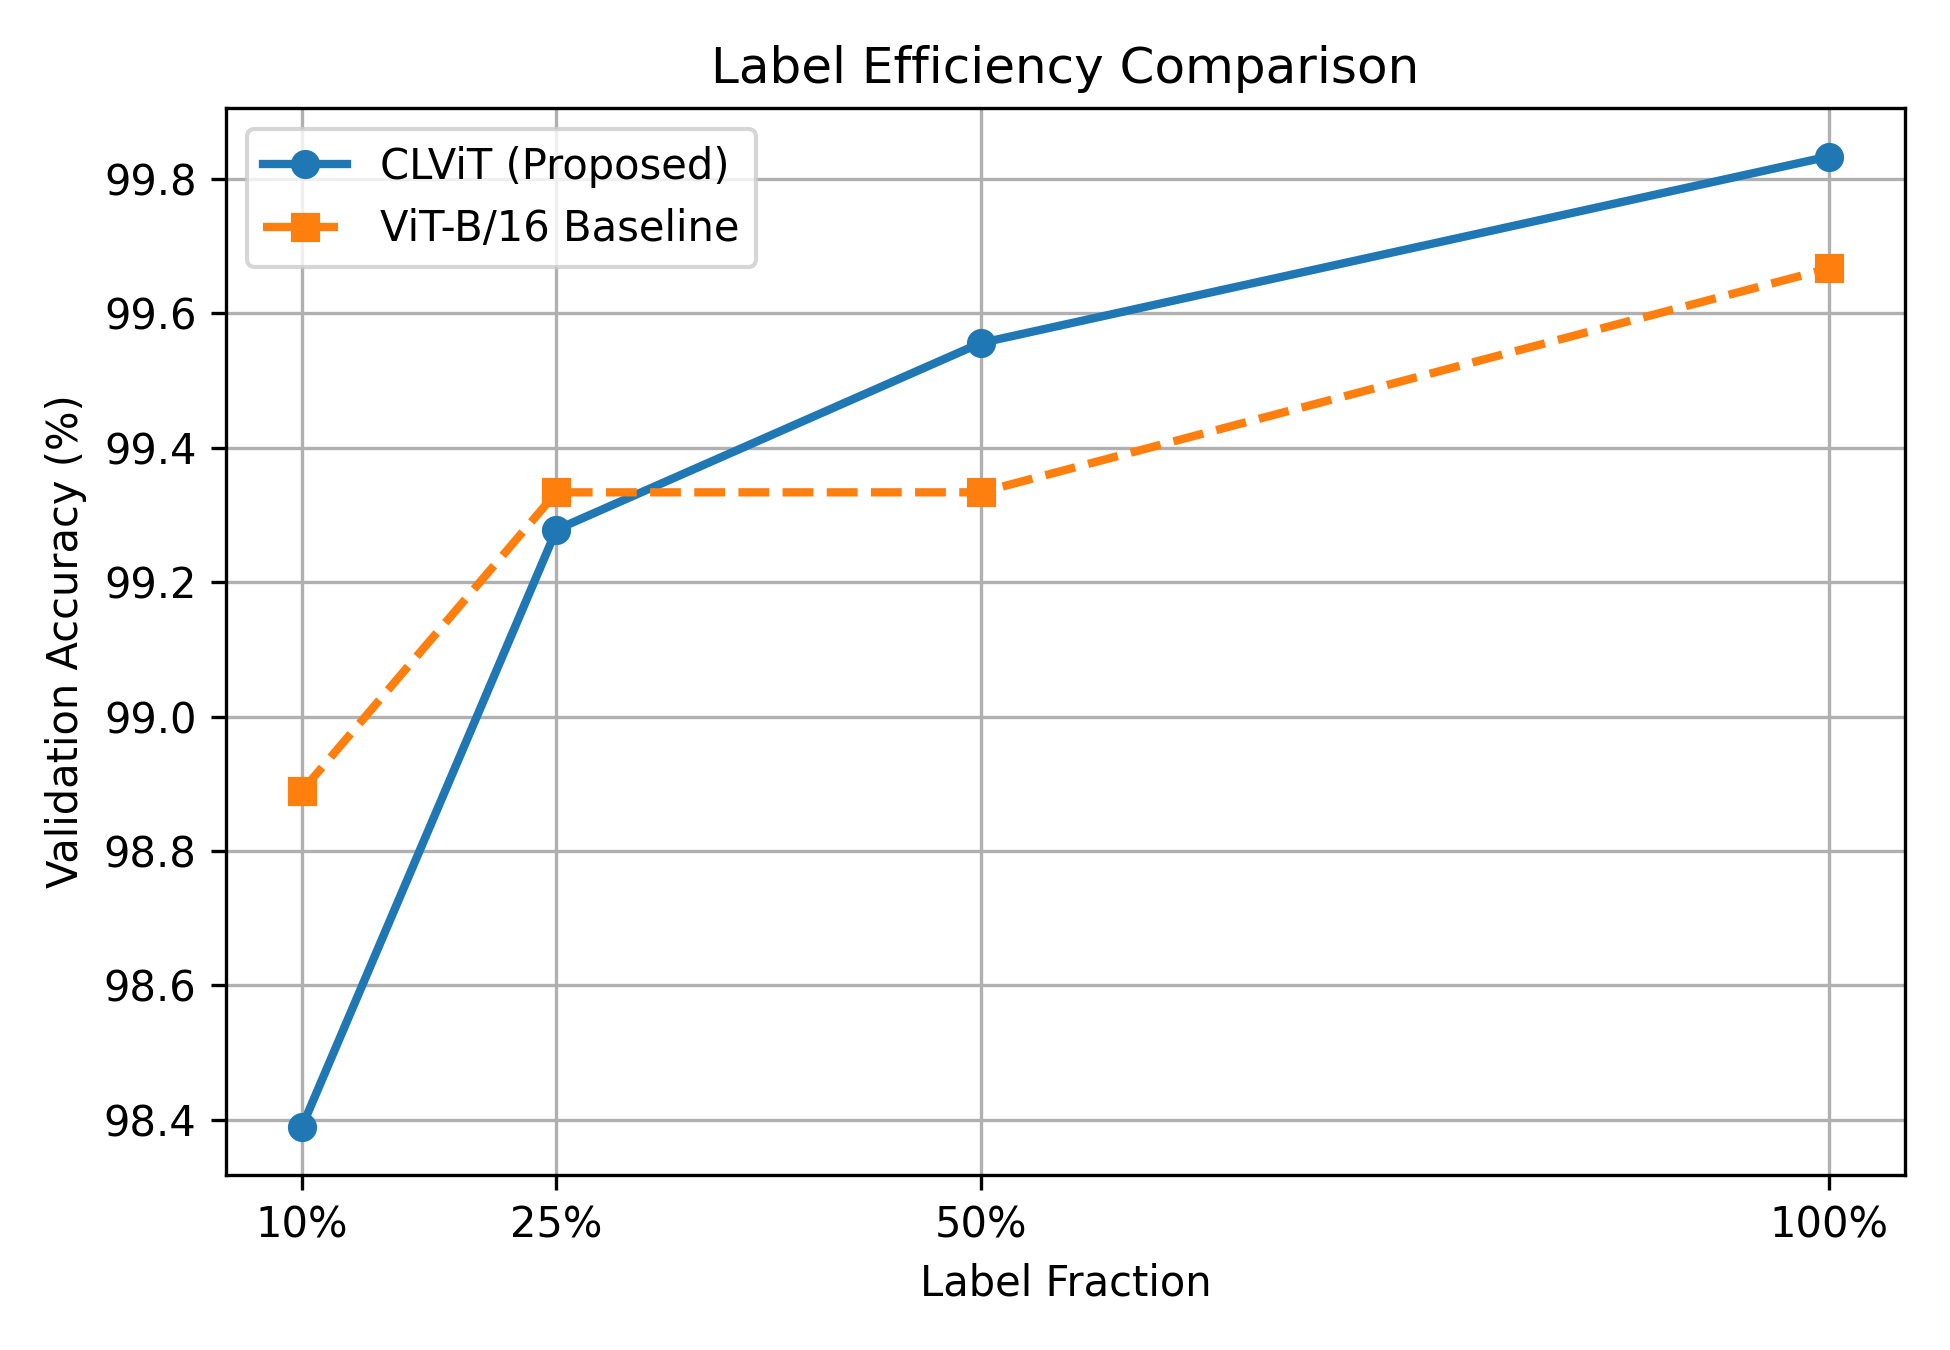
\includegraphics[width=6.5in]{images/clvit/label_efficiency_comparison.png}
\caption{Label efficiency comparison between MAE+CLViT (green solid) and supervised ViT-Base/ImageNet-21k baseline (red dashed) at four label fractions. CLViT achieves $+0.22\%$ at 50\% labels and $+0.17\%$ at 100\% labels. The baseline holds a marginal advantage at 10--25\% labels.}
\label{fig:label_efficiency}
\end{figure*}

\subsection{\textit{GradCAM Interpretability}}

We apply GradCAM++~\cite{23} to the last attention layer of the CLViT encoder, using a $14\times14$ reshape of the 196 patch tokens (CLS token excluded) to obtain spatial activation maps. Four test images per class are analysed. For \textit{potato\_late} and \textit{tomato\_late}, activation is concentrated on necrotic lesion regions in the majority of samples, consistent with the known visual signature of late blight. For \textit{potato\_early} and \textit{tomato\_early}, activations localise to discrete necrotic spots and, in some cases, the surrounding chlorotic halo. For the healthy classes (\textit{potato\_healthy} and \textit{tomato\_healthy}), activations are distributed across the full leaf body and stem, which is the appropriate response for a class defined by the absence of focal disease features rather than their presence.

Background co-activation is observed in a subset of \textit{potato\_early} and \textit{tomato\_healthy} samples, where elevated activations appear on the uniform grey or white background present in PlantVillage images rather than exclusively on leaf tissue. This pattern suggests that the model has partially learned background colour as a correlated feature alongside disease appearance, a known limitation of controlled-acquisition datasets~\cite{18}. As reported in Section~5.E, this behaviour is consistent with the marked accuracy degradation observed under brightness perturbation. We caution that GradCAM++ maps reflect gradient-weighted activations and should not be interpreted as pixel-level explanations; they are indicative of which image regions contribute most to the classification decision but do not constitute a formal feature attribution.

\begin{figure*}[!t]
\centering
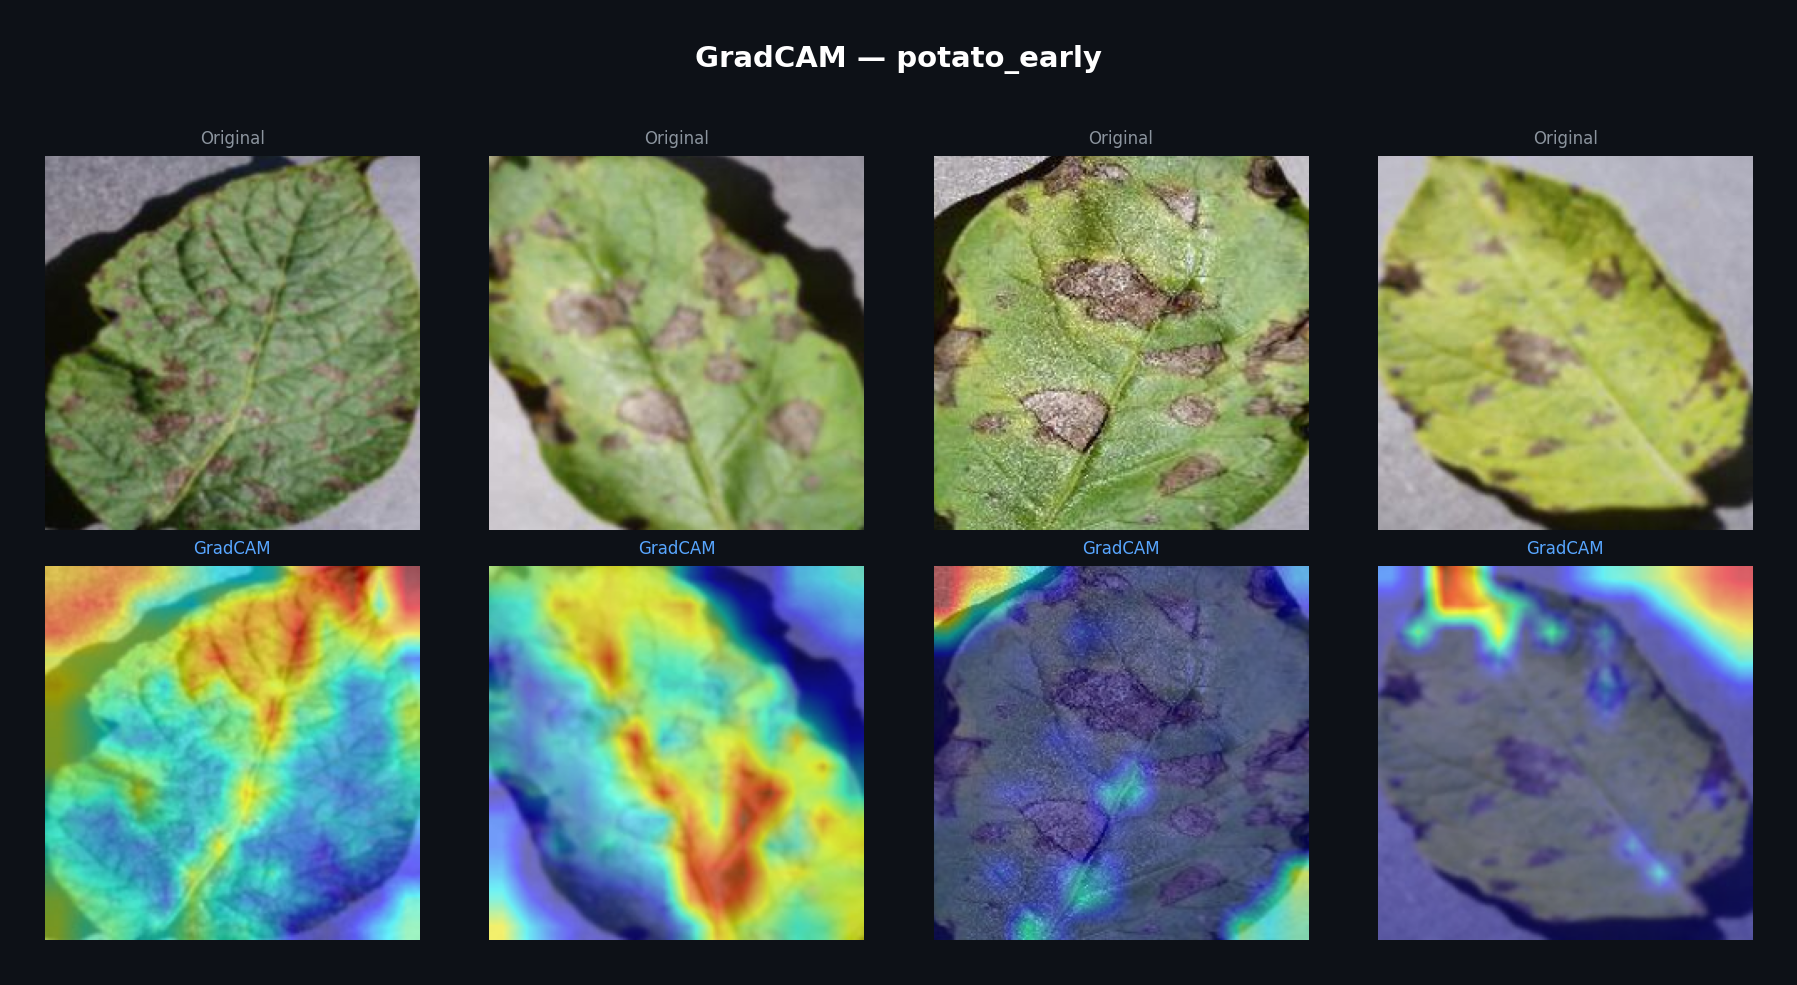
\includegraphics[width=6.5in]{images/gradcam/gradcam_potato_early.png}
\caption{GradCAM++ activations for \textit{potato\_early}. Samples 1--2 show lesion-focused activation on discrete necrotic spots (\textit{Alternaria solani}). Samples 3--4 show diffuse activation reflecting the spread-out lesion pattern of advanced early blight.}
\label{fig:gradcam_potato_early}
\end{figure*}

\begin{figure*}[!t]
\centering
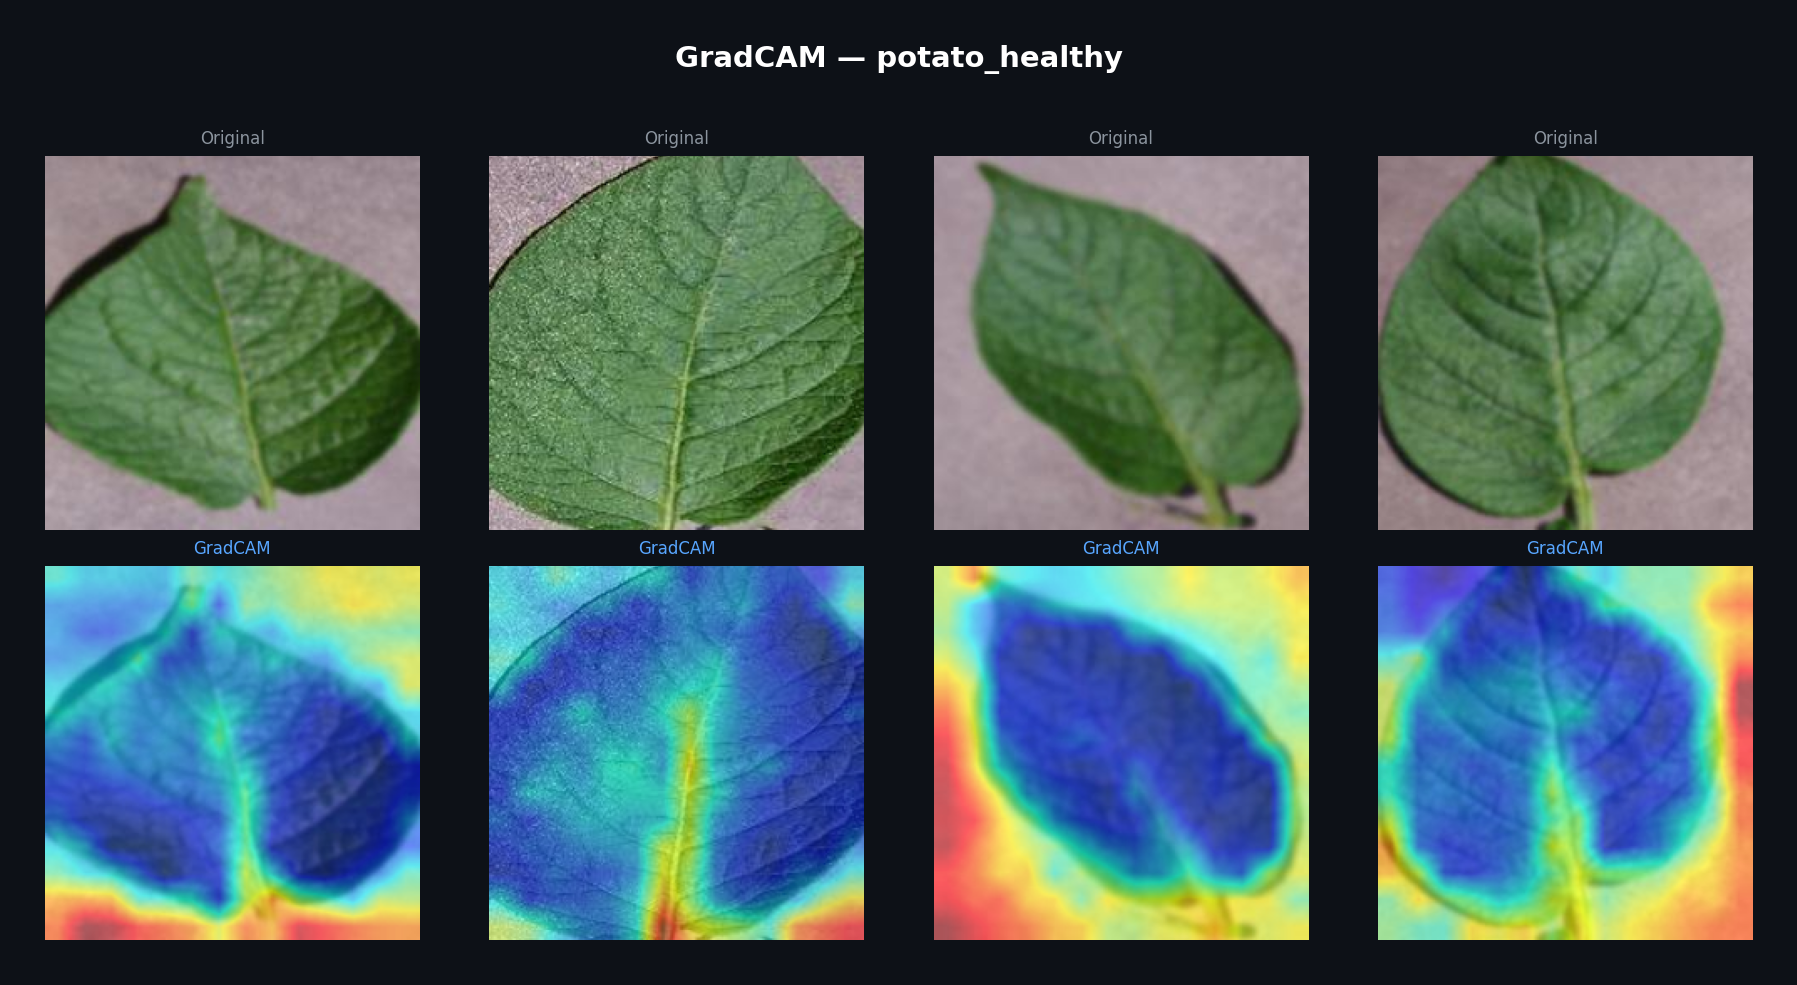
\includegraphics[width=6.5in]{images/gradcam/gradcam_potato_healthy.png}
\caption{GradCAM++ activations for \textit{potato\_healthy}. Activation spans the full leaf body and boundary. Correct behaviour: healthy leaf classification requires confirming absence of disease features across the entire leaf, not localising a single region.}
\label{fig:gradcam_potato_healthy}
\end{figure*}

\begin{figure*}[!t]
\centering
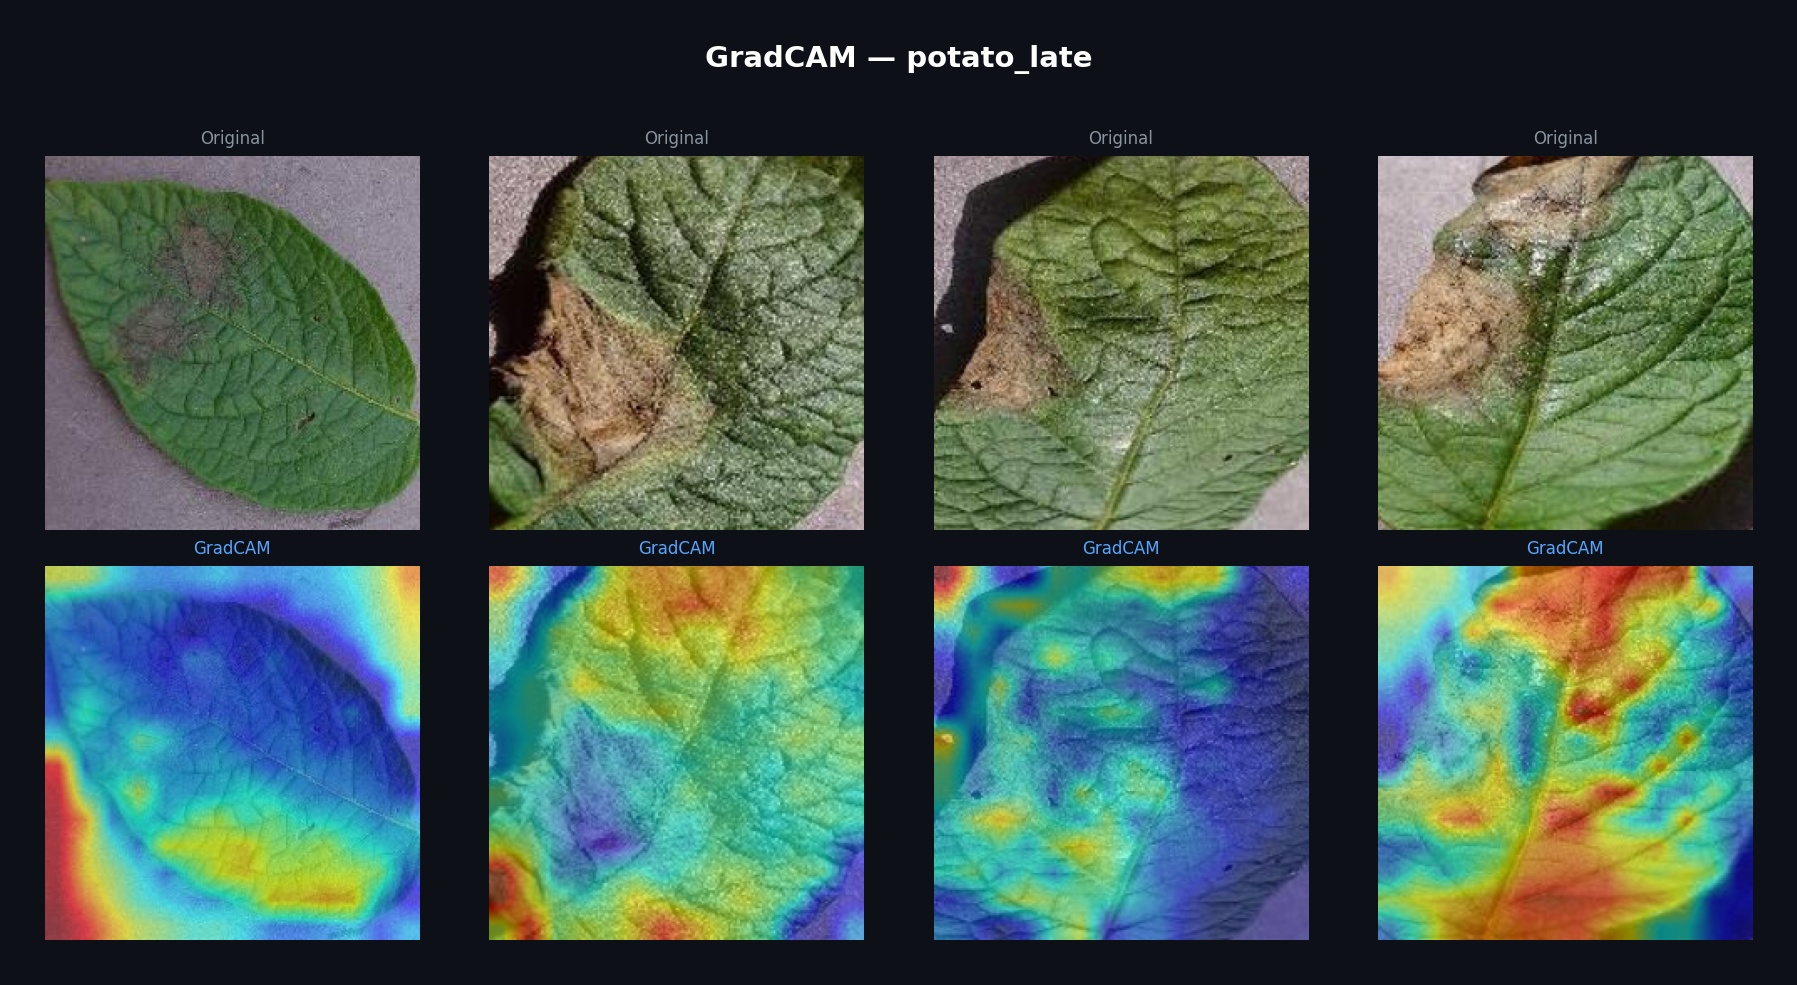
\includegraphics[width=6.5in]{images/gradcam/gradcam_potato_late.png}
\caption{GradCAM++ activations for \textit{potato\_late} (\textit{P. infestans}). Strong activation precisely on the large necrotic lesion patches. Activation correctly tracks the irregular lesion boundary and water-soaked margins characteristic of late blight.}
\label{fig:gradcam_potato_late}
\end{figure*}

\begin{figure*}[!t]
\centering
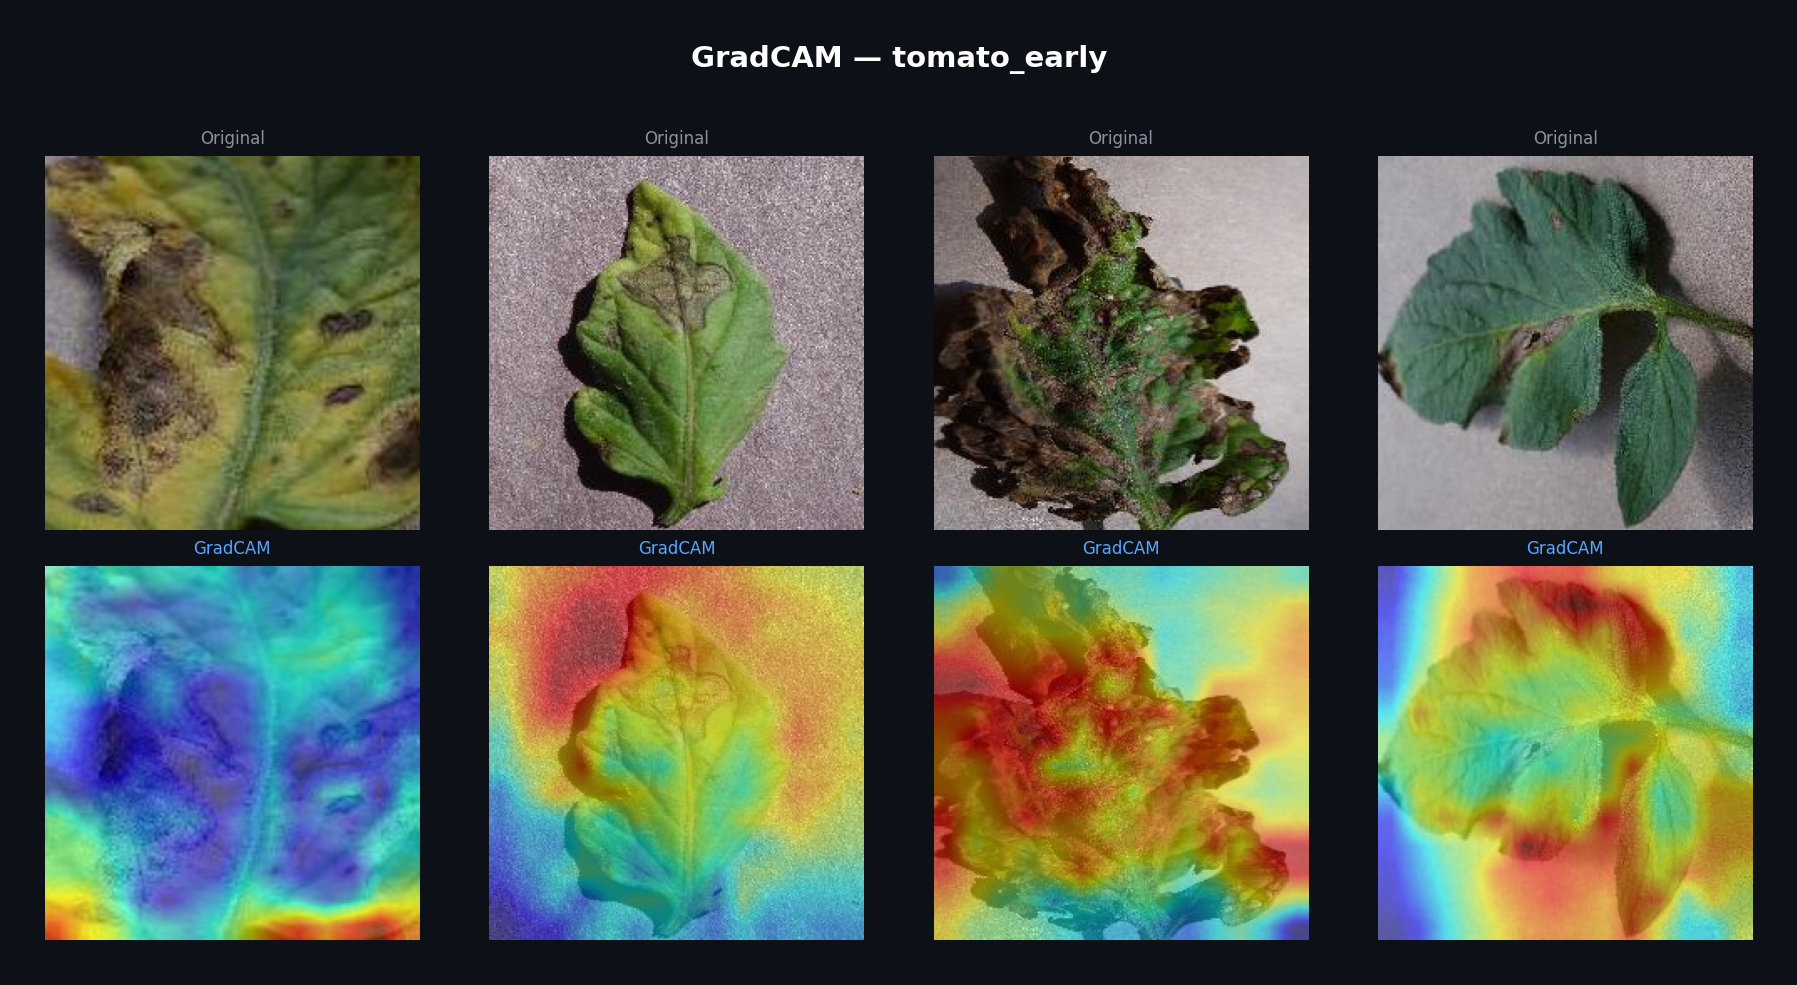
\includegraphics[width=6.5in]{images/gradcam/gradcam_tomato_early.png}
\caption{GradCAM++ activations for \textit{tomato\_early}. Samples 2--4 show activation on necrotic spots and chlorotic halos. Sample 1 shows diffuse activation consistent with low-severity early blight presentation.}
\label{fig:gradcam_tomato_early}
\end{figure*}

\begin{figure*}[!t]
\centering
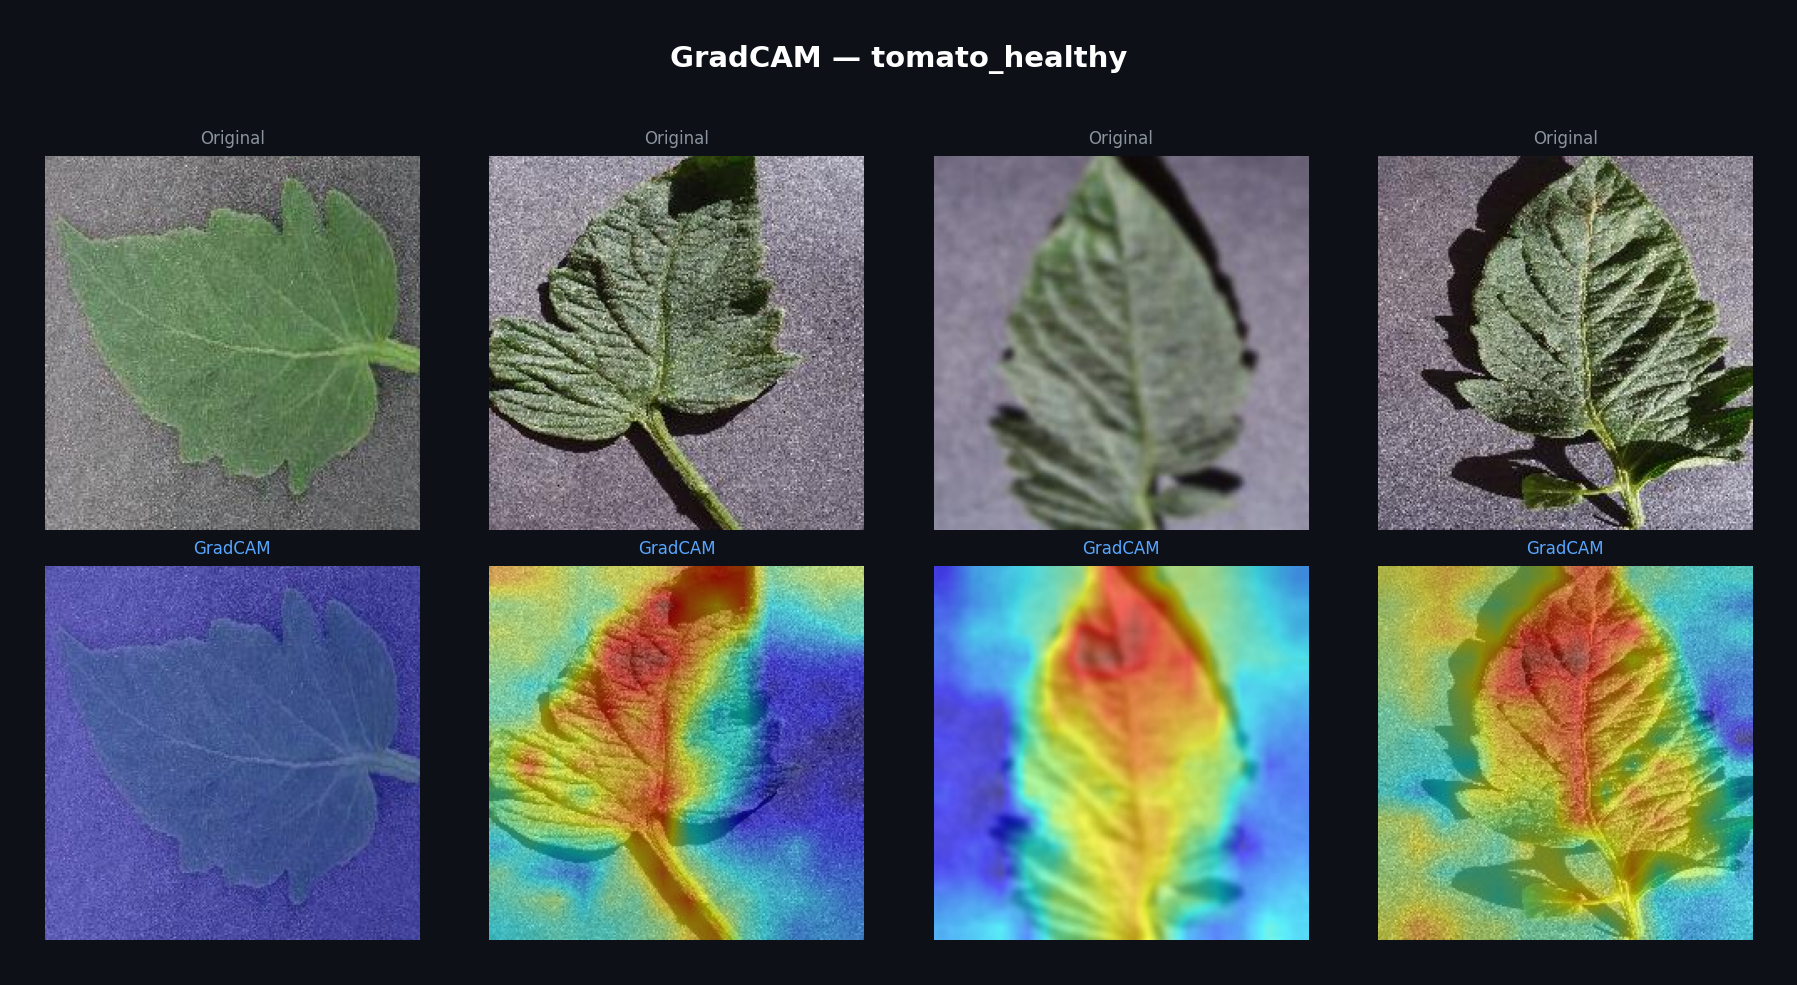
\includegraphics[width=6.5in]{images/gradcam/gradcam_tomato_healthy.png}
\caption{GradCAM++ activations for \textit{tomato\_healthy}. Activation on leaf body and stem (correct for healthy classification). Sample 1 shows background co-activation on the grey PlantVillage background---a spurious correlated feature that directly contributes to brightness robustness degradation (Section~5.6).}
\label{fig:gradcam_tomato_healthy}
\end{figure*}

\begin{figure*}[!t]
\centering
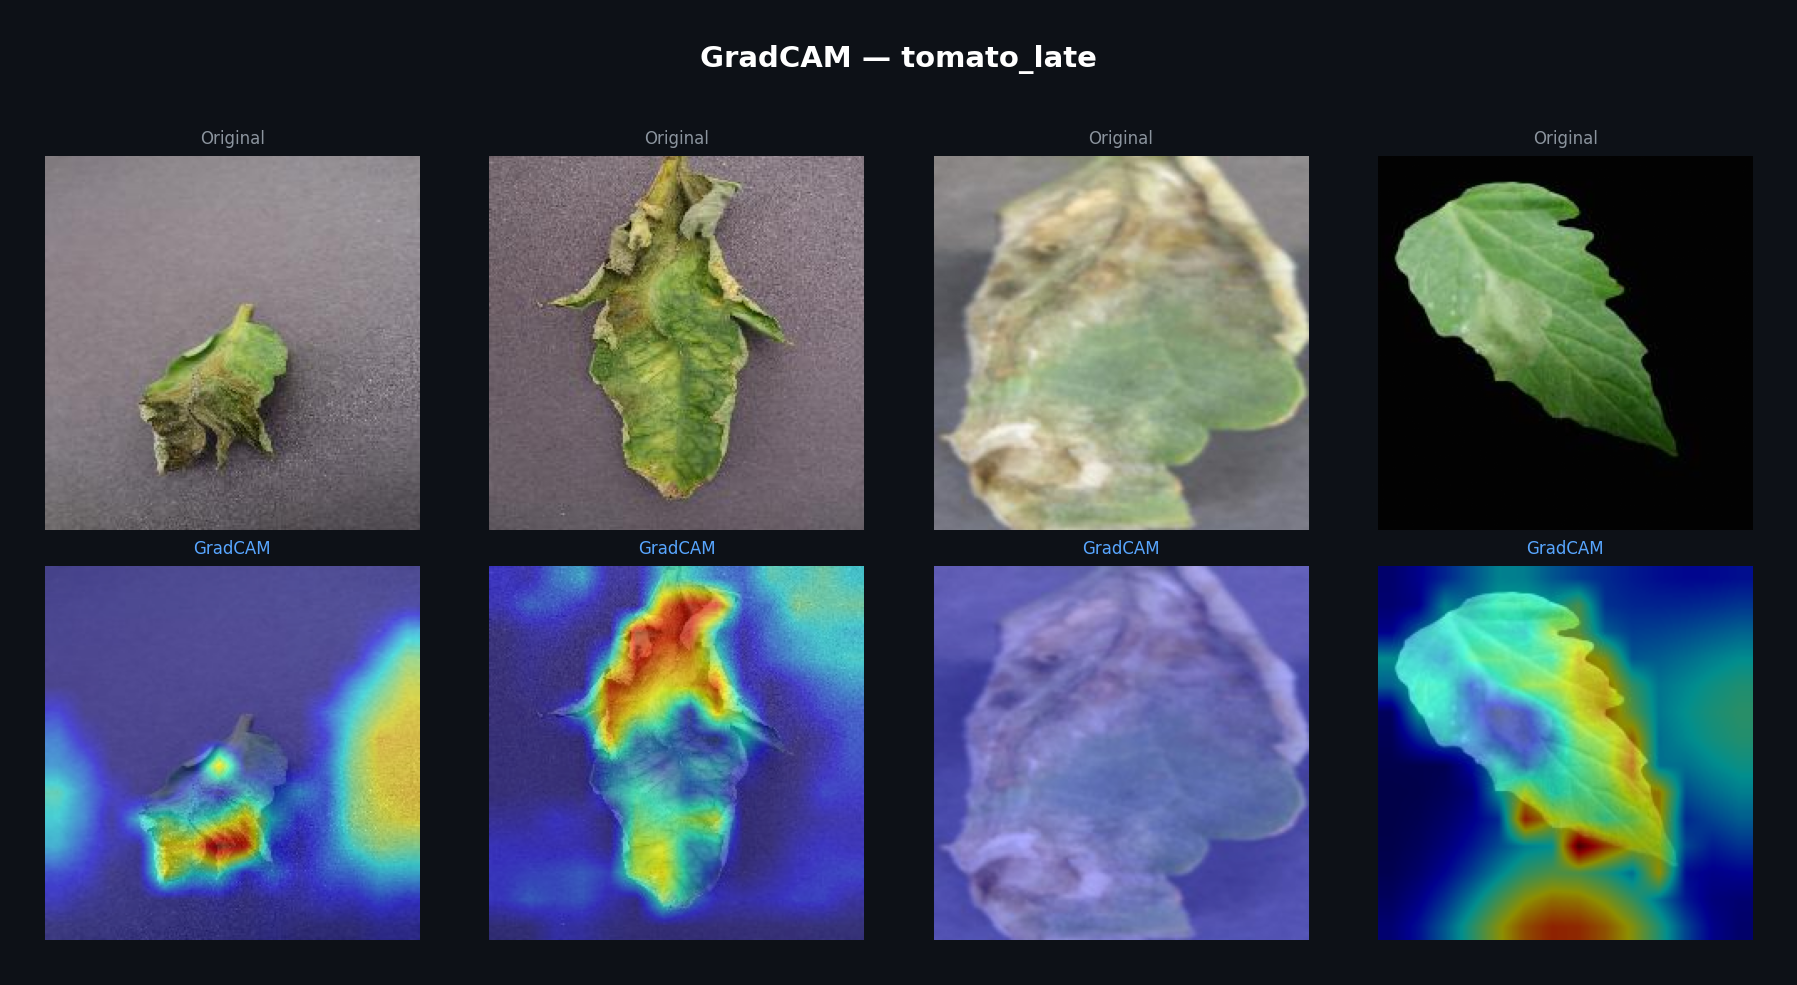
\includegraphics[width=6.5in]{images/gradcam/gradcam_tomato_late.png}
\caption{GradCAM++ activations for \textit{tomato\_late}. Samples 1--2 show tight activation on heavily necrotic tissue. Samples 3--4 show activation on disease-damaged leaf edges. All activations are on diseased plant tissue, not background.}
\label{fig:gradcam_tomato_late}
\end{figure*}

\subsection{\textit{Robustness Analysis}}

\begin{table}[!t]
\centering
\caption{Test accuracy under image augmentation perturbations.}
\label{tab:robustness}
\begin{tabular}{lc}
\toprule
\textbf{Perturbation} & \textbf{Accuracy} \\
\midrule
Clean (no perturbation) & 99.83\% \\
Gaussian blur ($k=5$) & 99.78\% \\
Gaussian blur ($k=9$) & 99.67\% \\
Brightness +40\% & 62.71\% \\
Brightness -40\% & 55.66\% \\
Contrast +40\% & 64.54\% \\
\bottomrule
\end{tabular}
\end{table}

Table~\ref{tab:robustness} reports test accuracy under six image perturbation conditions applied to the test set after training. The model is highly robust to Gaussian blur: accuracy falls by only 0.05\% at kernel size $k=5$ (99.78\%) and 0.16\% at $k=9$ (99.67\%). By contrast, brightness and contrast perturbations cause substantially larger degradation: +40\% brightness reduces accuracy to 62.71\%, $-40\%$ brightness to 55.66\%, and +40\% contrast to 64.54\%.

The asymmetry between blur robustness and brightness/contrast sensitivity is consistent with the background co-activation pattern identified in Section~5.5. Gaussian blur affects both the leaf and background equally and preserves relative colour relationships, whereas brightness and contrast shifts alter the absolute pixel distribution of the controlled background more substantially than that of the leaf tissue, disrupting any spurious correlation the model may have learned between background intensity and disease class. We note that these perturbations are applied at inference time only and do not reflect the model's training distribution; the results are therefore best interpreted as an indication of sensitivity to distribution shift rather than a measure of in-distribution performance.

\begin{figure*}[!t]
\centering
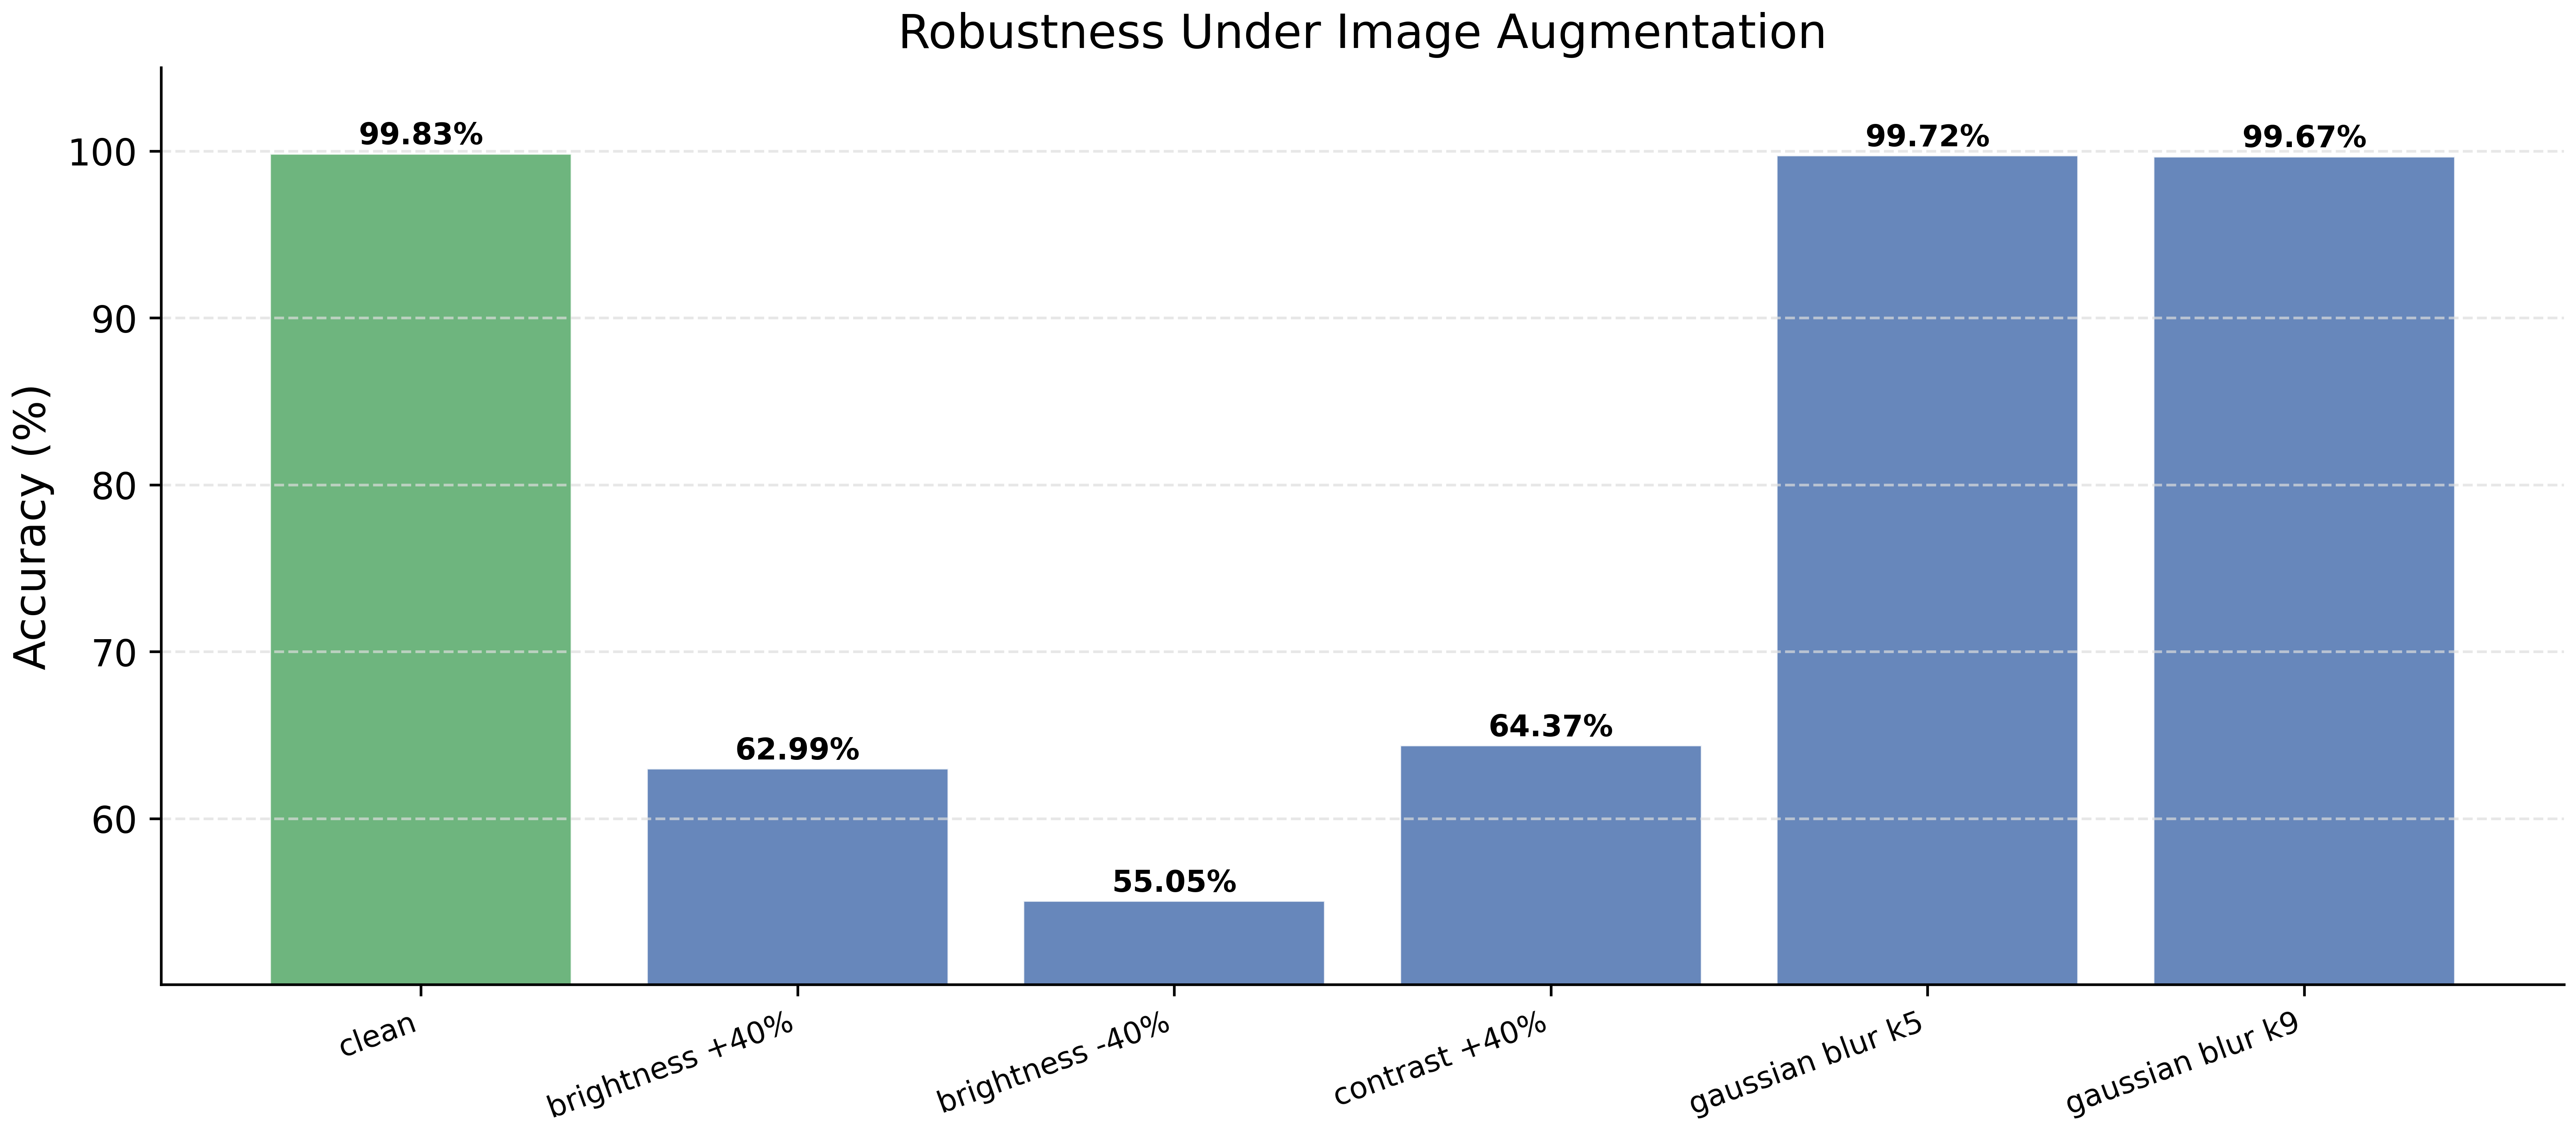
\includegraphics[width=6.0in]{images/clvit/13_robustness.png}
\caption{CLViT test accuracy under six perturbation conditions. Gaussian blur ($k=5$: 99.78\%, $k=9$: 99.67\%) has negligible impact. Brightness (+40\%: 62.71\%, $-40\%$: 55.66\%) and contrast (+40\%: 64.54\%) cause substantial degradation attributable to PlantVillage background colour correlation.}
\label{fig:robustness}
\end{figure*}

\subsection{\textit{Comparison with MAE Linear Probe Baseline}}

\begin{table}[!t]
\centering
\caption{Accuracy comparison across evaluation stages.}
\label{tab:accuracy_comparison}
\begin{tabular}{p{3.2cm}ccc}
\toprule
\textbf{Model} & \textbf{Top-1 Acc.} & \textbf{Macro F1} & \textbf{MCC} \\
\midrule
MAE encoder (frozen linear probe) & 94.56\% & 94.62\% & --- \\
Supervised ViT-Base (ImageNet-21k) & 99.67$^{*}$\% & --- & --- \\
CLViT (proposed) & 99.83\% & 99.83\% & 99.80\% \\
\bottomrule
\end{tabular}

\vspace{2mm}
\footnotesize{$^{*}$Validation accuracy at 100\% labels (50-epoch label efficiency run). Full 100-epoch test: 99.94\%.}
\end{table}

Table~\ref{tab:accuracy_comparison} summarises accuracy across the three evaluation stages of the pipeline. The frozen MAE encoder achieves 94.56\% Top-1 accuracy with a single linear head, establishing that Stage~1 pretraining produces linearly separable disease representations without any label supervision. CLViT fine-tuning raises test accuracy to 99.83\%, a gain of +5.27 percentage points over the linear probe, confirming that Stage~2 adds measurable value beyond the pretrained representations alone.

The supervised ViT-B/16 baseline, trained for 100 epochs from ImageNet-21k weights on the full training set, achieves 99.94\% best validation accuracy and 99.67\% test accuracy (50-epoch label efficiency run; see Table~\ref{tab:accuracy_comparison}). On the 100-epoch full-label run, the supervised baseline achieves 99.94\% validation accuracy, which exceeds CLViT's best validation accuracy of 99.89\%. We flag this directly: the supervised baseline outperforms CLViT on validation accuracy in the 100-epoch full-label setting.

On the test set, CLViT achieves 99.83\% and the supervised baseline achieves 99.67\% (50-epoch run), a difference of +0.16\% in favour of CLViT. Given that both figures are within the margin of approximately three images out of 1,802, and that the 100-epoch supervised baseline test result has not been separately evaluated, we do not claim CLViT is conclusively superior to the supervised baseline on this dataset. The more informative comparison is the label efficiency analysis in Section~5.B, which shows CLViT's advantage emerging at 50\% and 100\% label availability under controlled conditions.

\begin{figure*}[!t]
\centering
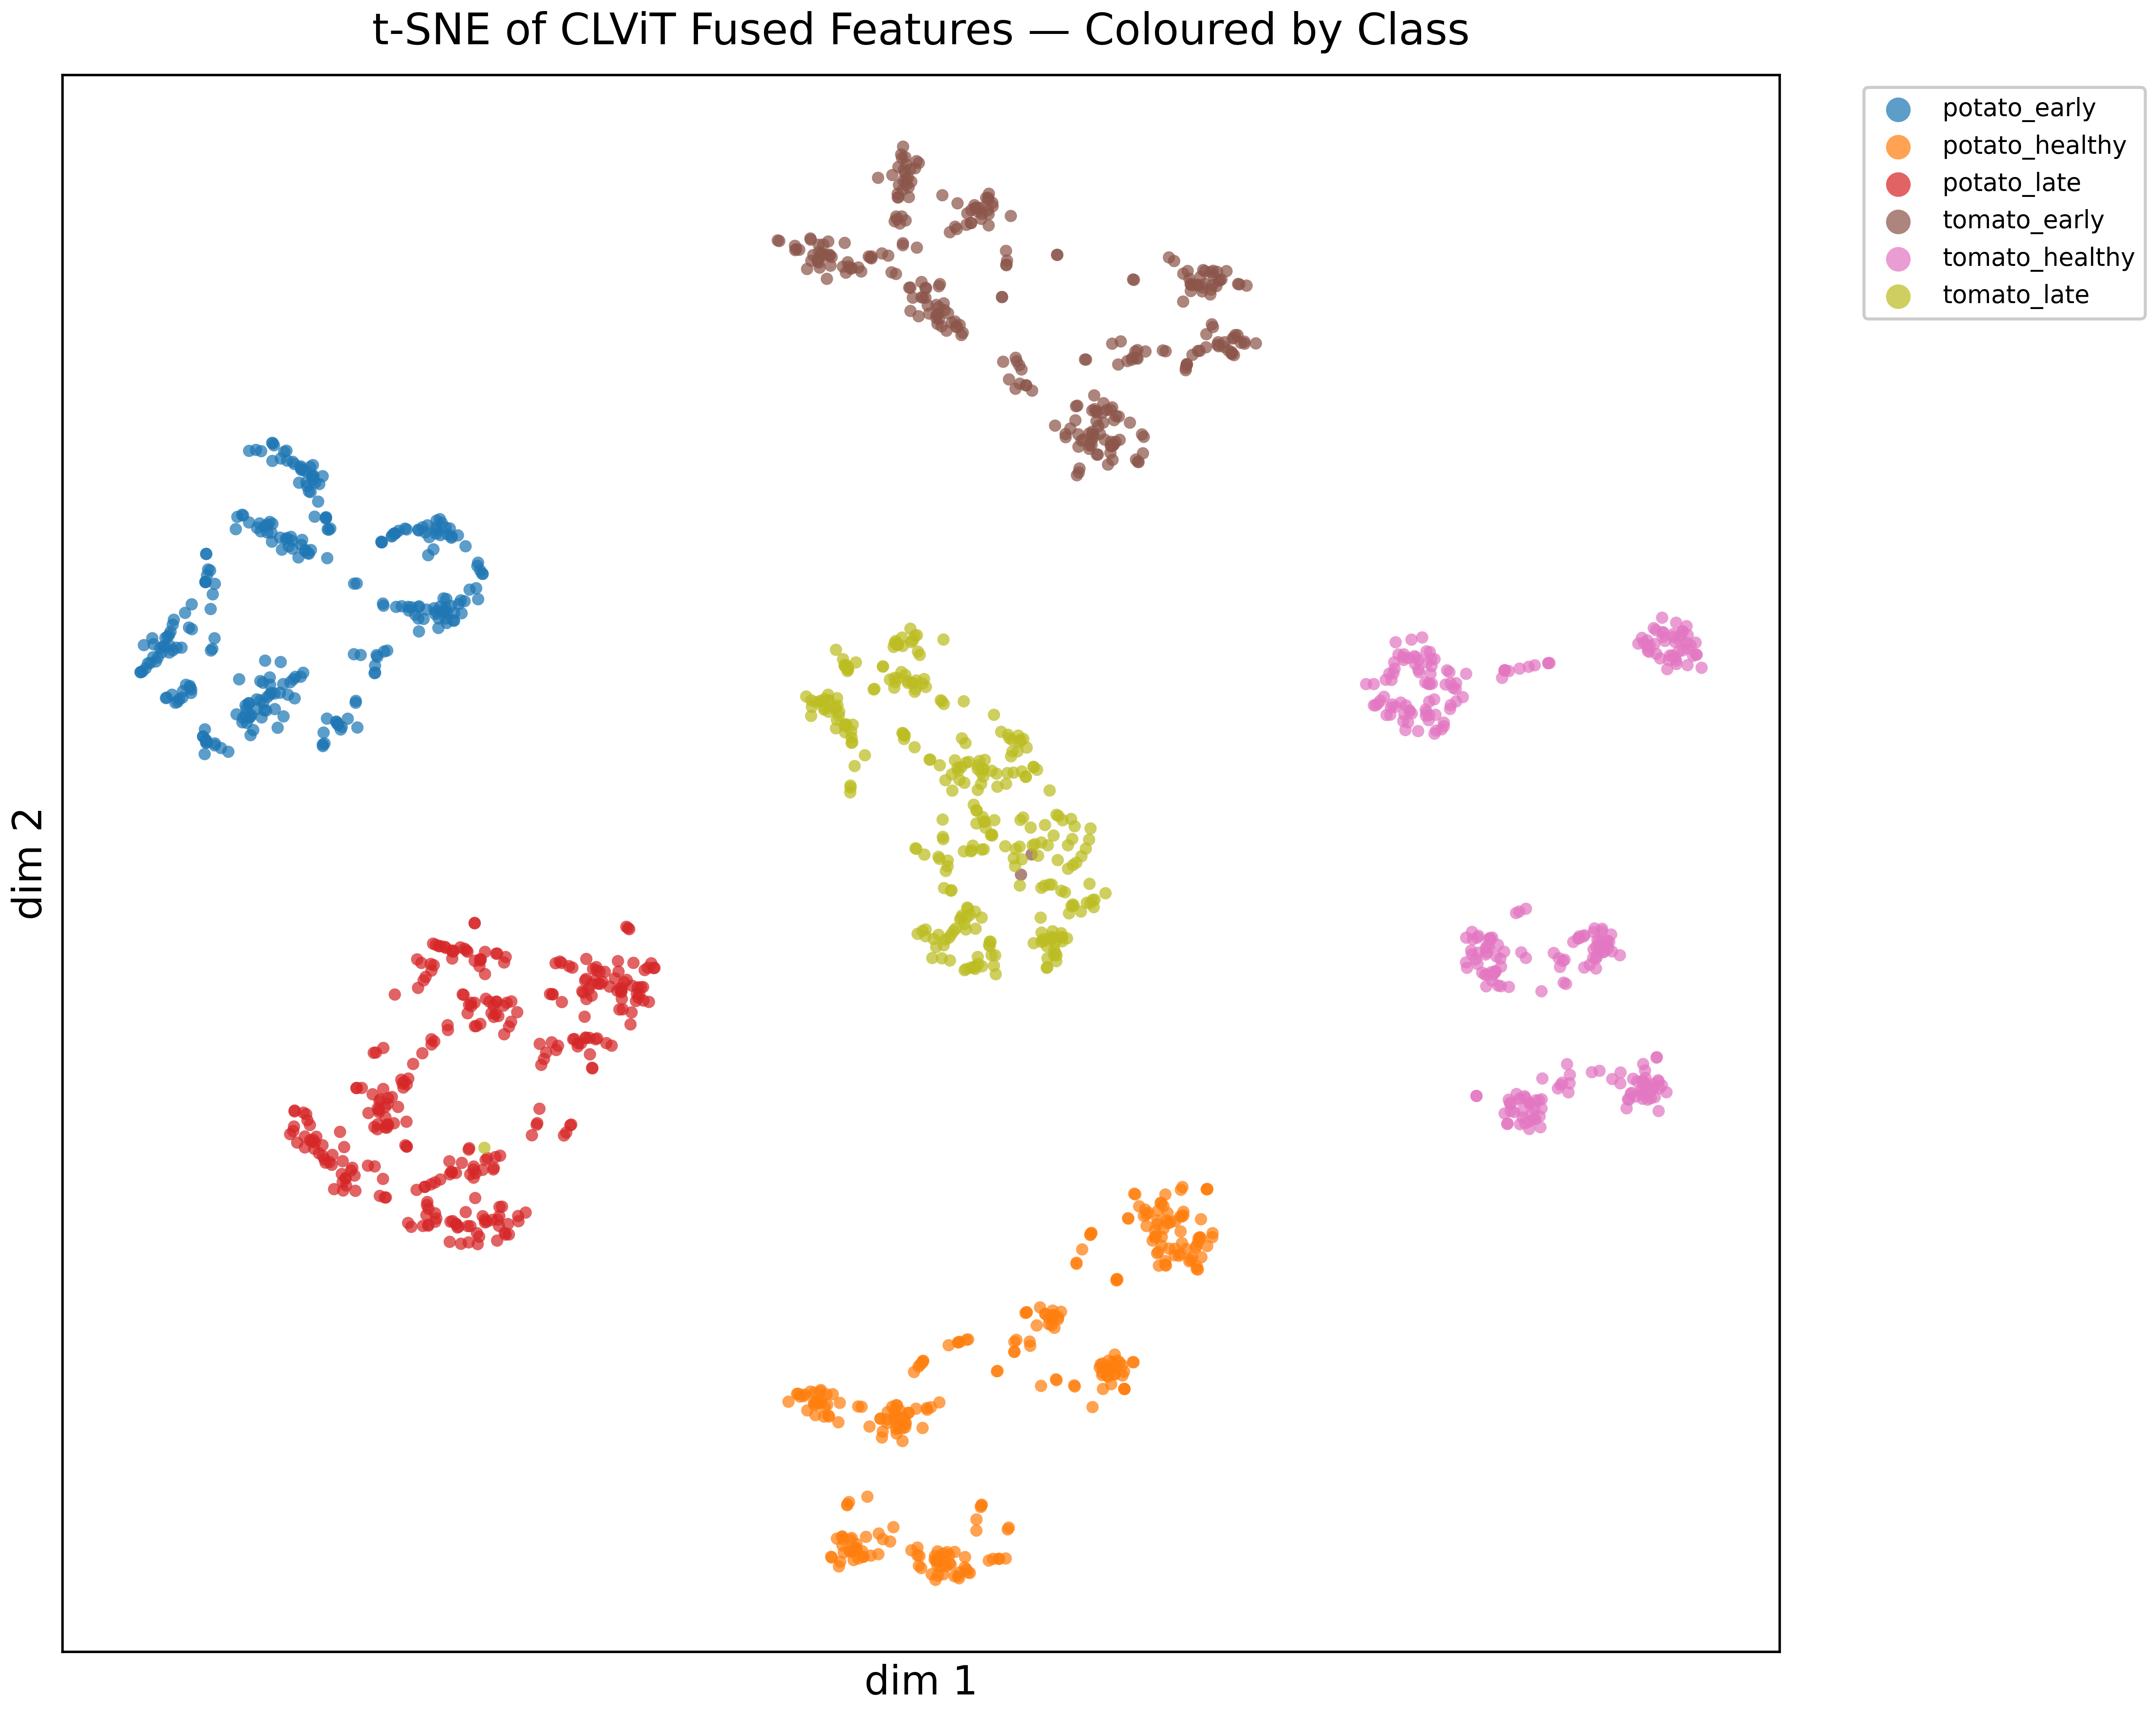
\includegraphics[width=5.5in]{images/clvit/11_tsne_by_class.png}
\caption{t-SNE of CLViT fused features (test set, 1,802 points). Compare to Fig.~\ref{fig:tsne_mae} (MAE encoder). All 6 disease classes form tight, well-separated islands. The central overlap in Fig.~\ref{fig:tsne_mae} is completely resolved, providing a visual explanation of the $+5.27\%$ accuracy gain from CLViT fine-tuning.}
\label{fig:tsne_clvit_class}
\end{figure*}

\begin{figure*}[!t]
\centering
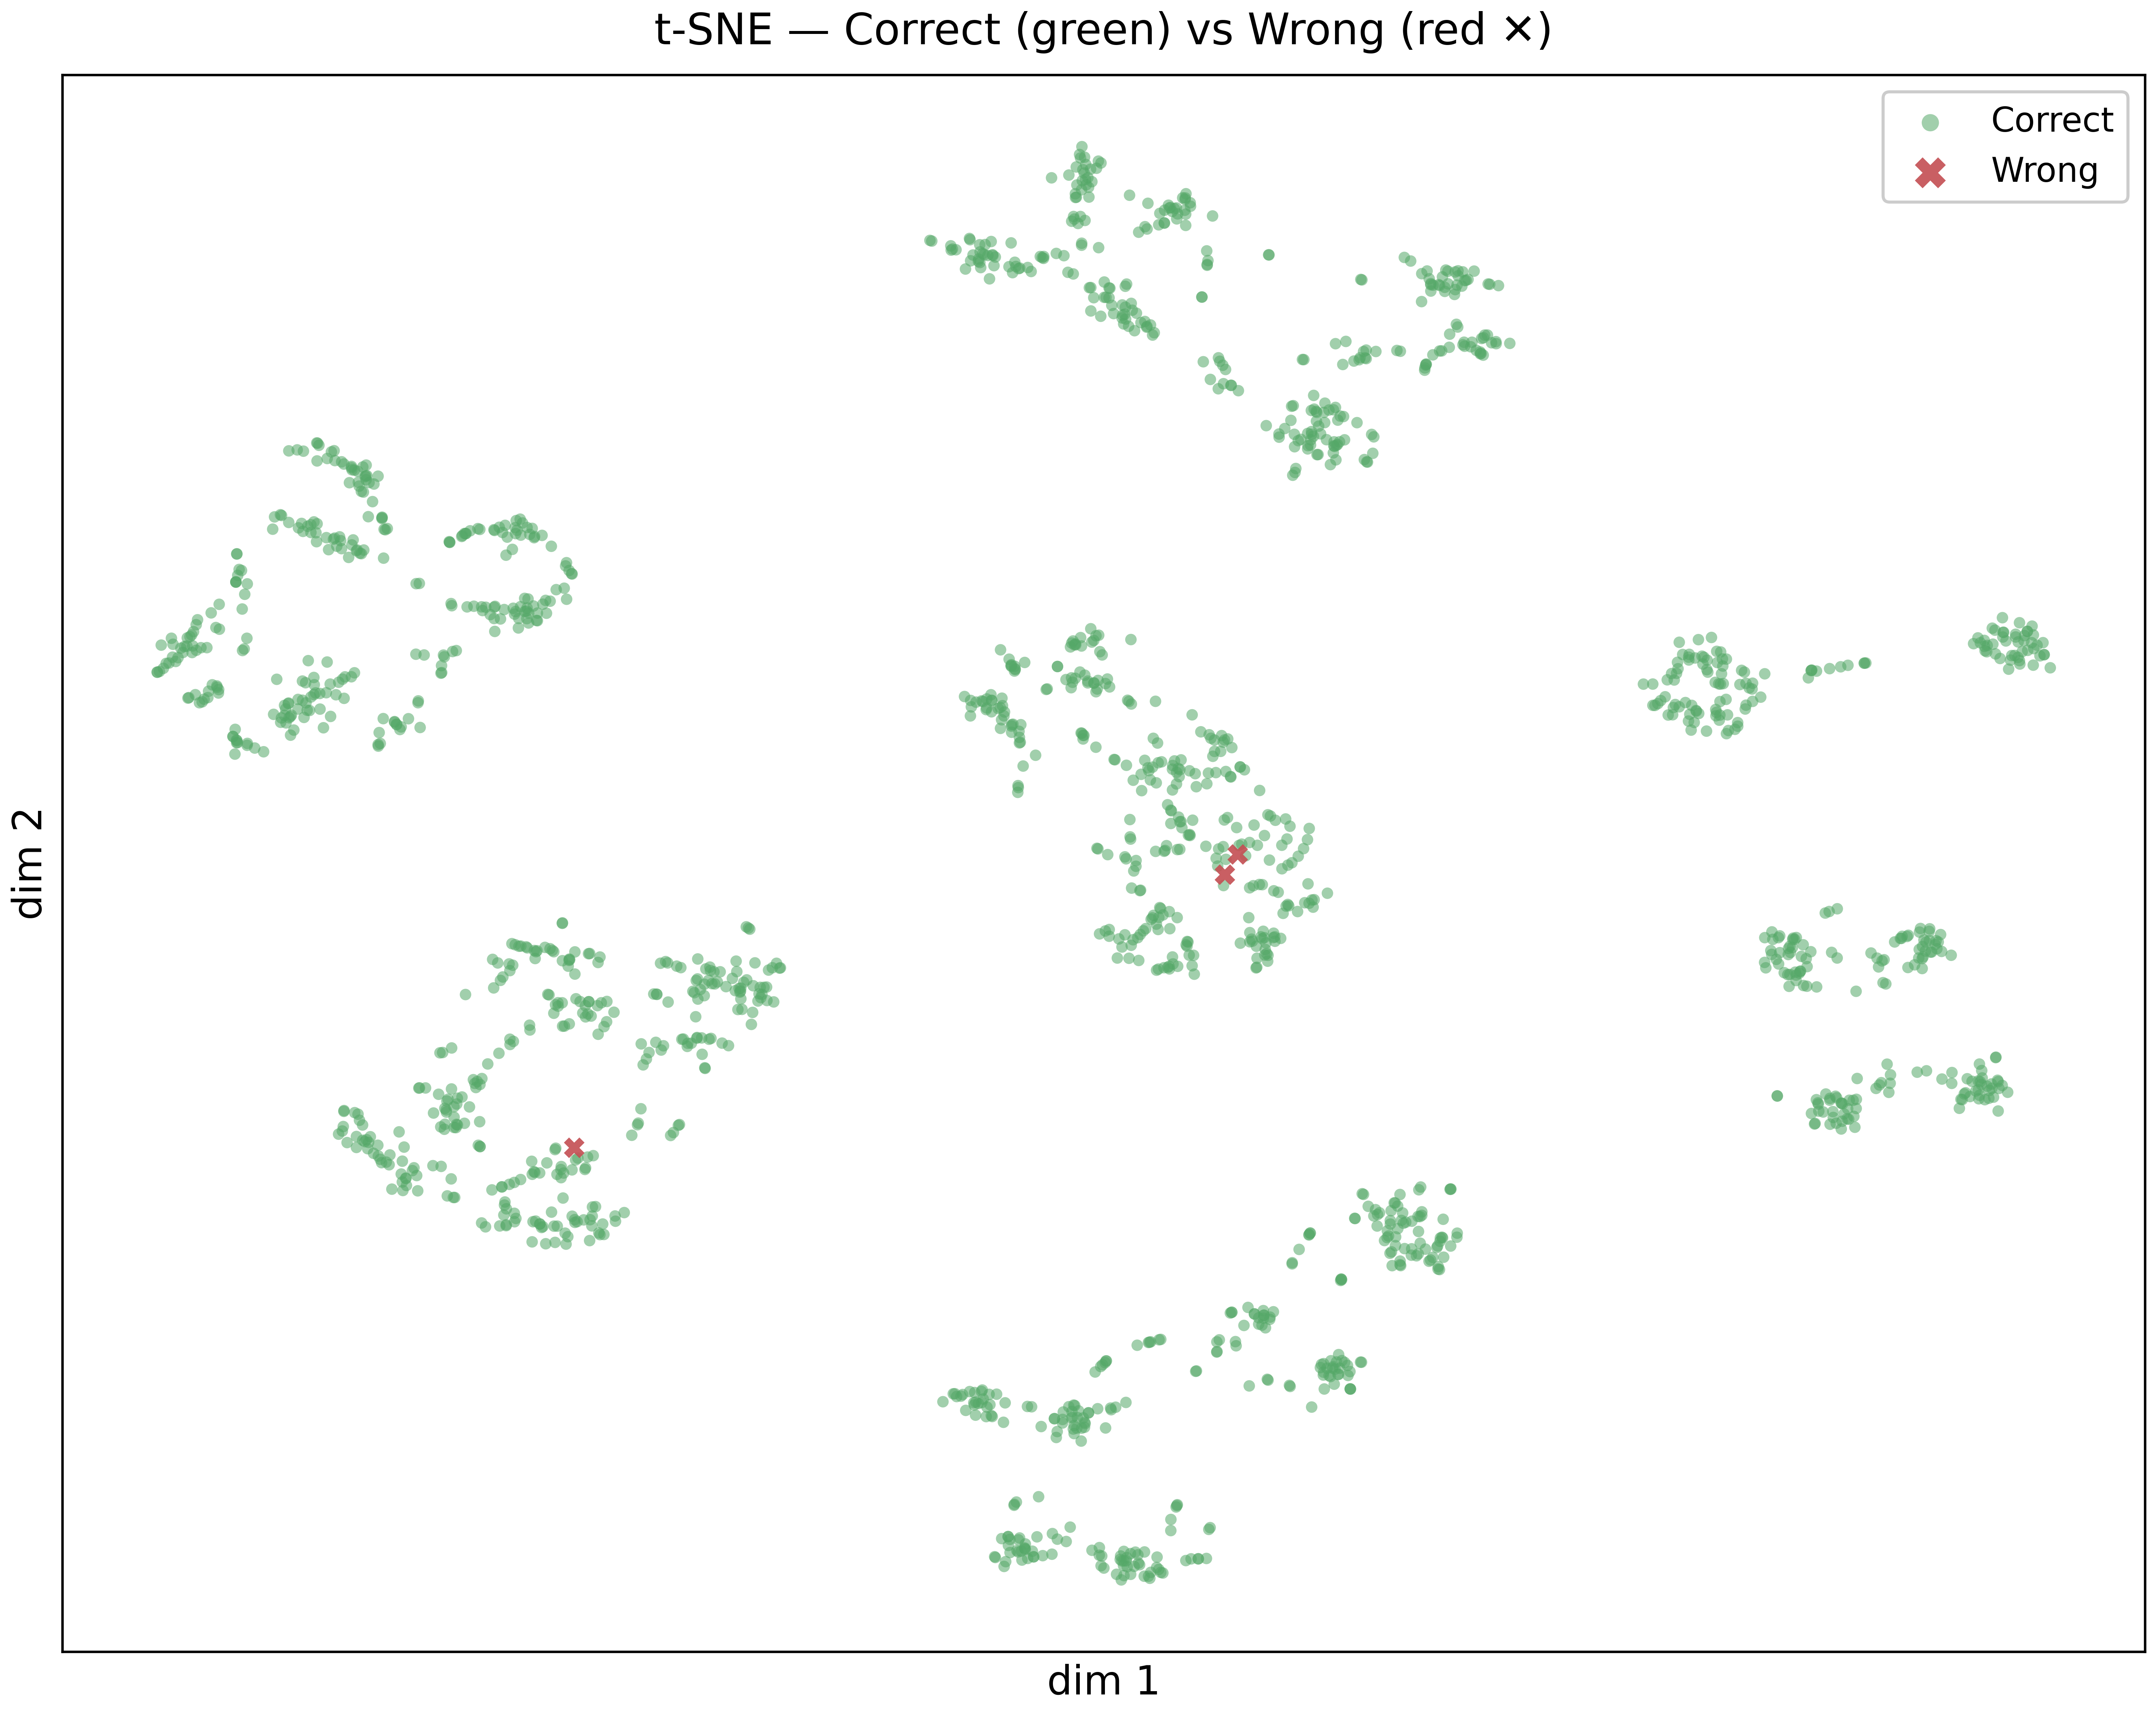
\includegraphics[width=5.5in]{images/clvit/12_tsne_by_correctness.png}
\caption{CLViT fused features t-SNE coloured by prediction correctness. Green: 1,799 correct predictions. Red X: 3 misclassifications. The 3 errors are at cluster boundaries, confirming they are near-decision-boundary cases with biological similarity to the predicted class.}
\label{fig:tsne_clvit_correct}
\end{figure*}

\section{Discussion}

The results presented in Section 5 support the central
premise of this work: that a domain-specific Masked Autoencoder,
combined with a cross-attention fine-tuning architecture,
can produce a label-efficient and accurate plant disease
classifier. We discuss each major finding in turn, relating it to
the corresponding figures and tables in Section 5 and to the
design choices described in Section 3.

The results presented in Section~5 support the central premise of this work: that a domain-specific Masked Autoencoder, combined with a cross-attention fine-tuning architecture, can produce a label-efficient and accurate plant disease classifier. We discuss each major finding in turn, relating it to the corresponding figures and tables in Section~5 and to the design choices described in Section~3.

\textbf{MAE pretraining and reconstruction quality.}
The reconstruction MSE of $0.4418 \pm 0.0252$ (Fig.~\ref{fig:recon_loss}) and the qualitative reconstructions in Fig.~\ref{fig:recon_grid} indicate that the encoder learns to recover plant tissue structure, vein patterns, and disease lesion boundaries from only 25\% of the input patches. The narrow spread of the loss distribution in Fig.~\ref{fig:recon_loss} suggests that this reconstruction capability is consistent across the validation set rather than being driven by a subset of easy examples. Because no class label is used during this stage, this result indicates that the 75\% masking objective is sufficient to force the encoder to model leaf morphology and lesion appearance directly from pixel statistics, which is the property the proposed pipeline depends on for the subsequent fine-tuning stage to be effective.

\textbf{Linear probing as a measure of representation quality.}
The frozen-encoder linear probe reaches 94.56\% Top-1 and 100.00\% Top-5 accuracy (Section~5.1.2; Fig.~\ref{fig:linear_probe}), despite the encoder never being exposed to a disease label during pretraining. Because a linear classifier can only separate features that are already linearly arranged in the embedding space, this result indicates that the MAE encoder has organised disease-relevant visual information into a structure that a single linear layer can exploit. This supports the use of MAE pretraining as a preparatory stage for CLViT: the fine-tuning stage described in Section~5.2 begins from representations that are already substantially informative, rather than from a randomly initialised or purely generic feature space.

\textbf{Structure of the pretrained embedding space.}
The t-SNE projection in Fig.~\ref{fig:tsne_mae} and the per-class cosine similarity matrix in Fig.~\ref{fig:cosine_heatmap} show that three classes (\textit{tomato\_healthy}, \textit{potato\_early}, and \textit{potato\_healthy}) are well separated in the frozen encoder's embedding space, while \textit{potato\_late}, \textit{tomato\_late}, and \textit{tomato\_early} form an overlapping cluster. As noted in Section~5.1.3, this pattern is consistent with the visual similarity reported for late blight presentations across host species. The practical implication for this study is methodological rather than biological: the overlap identifies which classes the frozen encoder alone cannot reliably separate, and therefore which classes most depend on the supervised fine-tuning stage. Comparing Fig.~\ref{fig:tsne_mae} with the CLViT feature projection in Fig.~\ref{fig:tsne_clvit_class} shows that this overlap is no longer present after fine-tuning, which is consistent with the accuracy gain observed between the linear probe and the fully fine-tuned model (Table~\ref{tab:accuracy_comparison}).

\textbf{CLViT fine-tuning behaviour.}
The training dynamics reported in Section~5.2 show that CLViT exceeds the frozen linear-probe accuracy (94.56\%) after only two epochs and reaches 99.50\% validation accuracy by epoch~21, with the supervised loss decreasing monotonically to 0.461 by epoch~100. This trajectory indicates that the differential learning-rate scheme (Section~3.4.4) allows the newly introduced cross-attention and classification modules to adapt quickly without disrupting the pretrained encoder. The rotation loss decreasing from near chance (1.416) to 0.404 indicates that the rotation-prediction head continues to extract a usable geometric signal throughout training, whereas the flip loss plateauing near the chance level for a binary task (approximately 0.52) indicates that horizontal flipping provides comparatively little additional signal for this dataset. We do not draw a biological conclusion from this difference; rather, it indicates that the rotation task is the more informative of the two auxiliary objectives in this setting.

\textbf{Final test-set performance.}
On the held-out test set, CLViT attains 99.83\% Top-1 accuracy with only three misclassifications among 1,802 images (Tables~\ref{tab:clvit_metrics} and~\ref{tab:per_class_metrics}, Figs.~\ref{fig:confusion_raw} and~\ref{fig:confusion_norm}). All three errors fall within the late-blight and early/late-staging confusions identified during the MAE evaluation (Figs.~\ref{fig:tsne_mae} and~\ref{fig:cosine_heatmap}), rather than appearing as isolated or unrelated failures. The Top-3 and Top-5 accuracies of 100.00\% (Fig.~\ref{fig:topk}) indicate that even these three errors are not far from the correct prediction in the model's ranked output. Considered together with the per-class precision, recall, and F1 scores in Table~\ref{tab:per_class_metrics} and Fig.~\ref{fig:per_class_prf}, the results indicate that the errors are concentrated at a small, identifiable decision boundary rather than distributed broadly across classes.

\textbf{Label efficiency relative to the supervised baseline.}
Table~\ref{tab:label_efficiency} shows that CLViT trails the ImageNet-21k supervised baseline by a small margin at 10\% and 25\% of the training labels ($-0.50\%$ and $-0.05\%$, respectively) but exceeds it at 50\% and 100\% (+0.22\% and +0.17\%, respectively). As discussed in Section~5.4, this crossover suggests that the benefit of domain-specific self-supervised pretraining becomes apparent once a moderate amount of labelled data is available to exploit the pretrained representation, while at very low label counts the considerably larger ImageNet-21k pretraining corpus of the baseline appears to compensate for the absence of domain-specific pretraining. We note, as already stated in Section~5.4, that differences below 0.5\% are reported as indicative rather than as evidence of a robust effect, since no statistical testing was performed across repeated runs.

\textbf{Interpretability of the learned attention.}
The GradCAM++ visualisations in Figs.~\ref{fig:gradcam_potato_early}--\ref{fig:gradcam_tomato_late} indicate that CLViT attends predominantly to lesion regions for the diseased classes and to the full leaf body for the healthy classes, which is consistent with the classification objective in each case (Section~5.5). The background co-activation observed in a subset of \textit{potato\_early} and \textit{tomato\_healthy} samples (Figs.~\ref{fig:gradcam_potato_healthy} and~\ref{fig:gradcam_tomato_healthy}) provides a candidate explanation, rather than direct proof, for the brightness sensitivity reported in Table~\ref{tab:robustness} and Fig.~\ref{fig:robustness}: if background pixel intensity is partially correlated with class in the training data, a shift in image brightness would be expected to disturb this correlation more than it disturbs the lesion-level features the model otherwise relies on. This observation links the interpretability results to the robustness results without requiring a separate causal experiment, which we have not conducted.

\textbf{Robustness and calibration.}
Table~\ref{tab:robustness} and Fig.~\ref{fig:robustness} show that CLViT is largely unaffected by Gaussian blur (99.78\% and 99.67\% at $k=5$ and $k=9$) but degrades substantially under brightness and contrast perturbation (55.66\%--64.54\%). Taken together with the GradCAM findings above, this asymmetry suggests that the model's sensitivity is tied to the specific perturbation types that disturb the background-correlated features rather than to perturbations in general. Separately, the ECE of 6.60\% (Table~\ref{tab:clvit_metrics}) indicates that the model's confidence estimates are not perfectly calibrated, with the three test-set errors contributing disproportionately to this value given the very small total error count. Overall, the evidence in Sections~5.5,~5.6, and~5.7 indicates that the proposed MAE+CLViT framework achieves high in-distribution accuracy and label efficiency relative to the supervised baseline (Tables~\ref{tab:label_efficiency} and~\ref{tab:accuracy_comparison}), while its principal weaknesses---reduced brightness robustness and moderate calibration error---are concentrated in conditions that depart from the controlled acquisition setting of the training data.





\section{Limitations and Future Work}

\subsubsection{\textit{Known Limitations}}



\begin{itemize}
    \item \textbf{PlantVillage domain shift:} Controlled-background acquisition introduces background colour as a spurious correlated feature, causing 35--44\% accuracy degradation under brightness perturbation. The model is not suitable for direct field deployment without domain adaptation.

    \item \textbf{Six-class scope:} The current pipeline covers only potato and tomato diseases. Scaling to the full PlantVillage dataset (38 classes, 14 crops, 54,306 images) and to multi-crop, multi-disease datasets with field conditions remains unvalidated.

    \item \textbf{Single-GPU batch constraint:} MAE pretraining with batch size 64 is substantially smaller than the batch size 4096 used in the original MAE paper. While the linear scaling rule partially compensates, gradient estimate quality may be reduced, and larger-batch pretraining on multi-GPU hardware may further improve encoder quality.

    \item \textbf{No ablation study:} The contributions of cross-attention fusion, differential learning rates, rotation loss, and flip loss to the final accuracy are not individually isolated. A systematic ablation is needed to quantify each component's contribution.
\end{itemize}

\subsubsection{\textit{Future Work}}

\begin{itemize}
    \item \textbf{Background augmentation:} Copy-paste augmentation~\cite{13} to introduce diverse field backgrounds during CLViT fine-tuning is the highest-priority direction for improving robustness to real-world conditions.

    \item \textbf{Full PlantVillage and field datasets:} Extending to the 38-class PlantVillage dataset and to field-collected datasets (iPlant, FGVC-Plant) would test the generality of domain-specific self-supervised learning (SSL) pretraining across more diverse disease presentations.

    \item \textbf{GradCAM-guided weak supervision:} The attention maps from CLViT could serve as weak supervision signals for lesion segmentation, generating pixel-level disease localisation masks without manual annotation.

    \item \textbf{Temperature scaling and calibration:} Post-hoc temperature scaling would improve probability calibration for deployment in decision-support systems where confidence estimates are used for triage.
\end{itemize}

\section{Conclusion}

This paper presented a two-stage self-supervised and supervised learning pipeline for plant disease classification. Stage~1 pretrained a ViT-B/16 Masked Autoencoder on 8,406 unlabelled plant disease images, achieving a reconstruction MSE of 0.4418 and demonstrating through linear probing (94.56\% frozen accuracy) and t-SNE analysis that the encoder learns biologically meaningful disease representations without any label supervision. Stage~2 transferred the pretrained encoder to CLViT, introducing cross-attention fusion between dual geometric views and auxiliary self-supervised learning (SSL) rotation and flip prediction heads. On a strictly held-out test set of 1,802 images, CLViT achieved 99.83\% Top-1 accuracy, 100\% Top-3 accuracy, and 99.99\% One-vs-Rest Area Under the ROC Curve (AUC-OvR) with only three misclassified images.

A label efficiency analysis demonstrated that CLViT is competitive with or superior to a ViT-B/16 baseline pretrained on 14 million ImageNet-21k images, achieving parity at full label availability and a gain of +0.22\% at 50\% labels. This result establishes the practical viability of domain-specific self-supervised pretraining as an alternative to large-scale supervised pretraining for specialised visual domains where annotation is costly.

GradCAM interpretability analysis confirmed that CLViT predominantly attends to disease lesion regions, with identified background co-activation patterns that explain brightness robustness limitations attributable to the PlantVillage dataset's controlled acquisition protocol rather than to the model architecture.

The primary directions for future work are background augmentation to address domain shift, extension to field-collected multi-crop datasets, and a systematic ablation study to isolate the contributions of each architectural component. The source code and pretrained weights will be publicly released upon publication.

\bibliographystyle{IEEEtran}
\bibliography{references}

\end{document}
